% =============================================================================
% Charla PhytoLearning (versión divulgación, público general)
% Geometría y LLMs para clases con pocos ejemplos
% Benjamín Schindler — Laboratorio Dr. Gonzalo Ruz, UAI — 31 de julio de 2026
% Adaptada desde la presentación de defensa (ver ../Presentacion_Defensa)
% Compilar con: xelatex (preferido) o lualatex
% =============================================================================

\documentclass[10pt,aspectratio=169]{beamer}

% --- Tema Metropolis con paleta UAI ---
\usetheme[
  progressbar=frametitle,
  sectionpage=progressbar,
  numbering=fraction,
  block=fill
]{metropolis}

% --- Paquetes base ---
\usepackage[spanish,es-tabla,es-noindentfirst]{babel}
\usepackage{fontspec}
\usepackage{amsmath,amssymb}
\usepackage{mathtools}
\usepackage{booktabs,multirow,multicol}
\usepackage{tikz}
\usetikzlibrary{shapes,arrows.meta,positioning,fit,calc,backgrounds,shadows.blur,patterns,decorations.pathreplacing}
\usepackage{graphicx}
\usepackage{xcolor}
\usepackage{colortbl}
\usepackage{tcolorbox}
\usepackage{appendixnumberbeamer}
\usepackage{pifont}
\usepackage{caption}
\captionsetup{font=scriptsize, labelfont={bf,scriptsize}}

% --- Fuente: Cantarell (similar a Fira Sans, instalada en sistema) ---
\setsansfont{Cantarell}[
  Extension       = .otf,
  UprightFont     = *-Regular,
  ItalicFont      = *-Regular,
  BoldFont        = *-Bold,
  BoldItalicFont  = *-Bold,
  Path            = /usr/share/fonts/opentype/cantarell/,
  Scale           = 0.95
]
\setmonofont{DejaVu Sans Mono}[Scale=0.85]

% --- Estilos custom UAI ---
\usepackage{style/uai-colors}
\usepackage{style/beamer-blocks}

% --- Configuración Metropolis adicional ---
\setbeamertemplate{section in toc}[sections numbered]
\metroset{titleformat=regular}

% --- Section page custom: título grande + indicador lateral ---
\setbeamertemplate{section page}{%
  \begin{centering}
  \vspace{0.3em}
  \begin{minipage}{0.94\textwidth}
    \begin{columns}[c]
      \begin{column}{0.52\textwidth}
        \raggedright
        {\color{uaiorange}\fontsize{42}{46}\selectfont\bfseries\thesecnum.}\\[0.3em]
        {\color{uaibluedark}\Large\bfseries\insertsectionhead}
      \end{column}
      \begin{column}{0.46\textwidth}
        \sectionnav{\value{secnum}}
      \end{column}
    \end{columns}
  \end{minipage}
  \end{centering}%
}
\AtBeginSection[]{%
  \stepcounter{secnum}%
  \begin{frame}[plain,c,noframenumbering]\sectionpage\end{frame}%
}

% --- Ruta de figuras ---
\graphicspath{{figuras/}{logos/}{img/}}

% --- Comandos abreviados ---
\newcommand{\dataset}[1]{\texttt{\small #1}}
\newcommand{\filter}[1]{\textit{#1}}
\newcommand{\good}{\textcolor{uaigreen}{\ding{51}}}
\newcommand{\bad}{\textcolor{uaiorange}{\ding{55}}}

% --- Información título ---
\title{Geometría y LLMs para clases con pocos ejemplos}
\subtitle{Cómo elegir datos generados por IA}
\author{\textbf{Benjamín Schindler}}
\institute{
  Laboratorio Dr. Gonzalo A. Ruz\\
  Master of Science in Data Science\\
  Universidad Adolfo Ibáñez\\[6pt]
  \footnotesize Reunión Mensual PhytoLearning
}
\date{31 de julio de 2026}
\titlegraphic{\hfill
\includegraphics[height=1.2cm]{logos/fic.png}}

% =============================================================================
\begin{document}

% --- Bloque 1: Apertura ---
% =============================================================================
% Bloque 1: Apertura (slides 1–2)
% =============================================================================

% --- Slide 1: Portada PhytoLearning (charla de divulgación) ---
\begin{frame}[plain,noframenumbering]
\vspace*{0.6em}
\begin{columns}[T,onlytextwidth]
%
\begin{column}{0.68\textwidth}
\raggedright
{\color{uaigray}\footnotesize Reunión Mensual \textbf{PhytoLearning}}

\vspace{1.1em}

{\color{uaibluedark}\fontsize{20}{24}\selectfont\bfseries Geometría y LLMs\\ para clases con pocos ejemplos}\\[0.55em]
{\color{uaigray}\small Cómo elegir datos generados por IA}

\vspace{1.0em}
{\color{uaiorange}\rule{0.52\textwidth}{1pt}}
\vspace{1.0em}

{\large\bfseries\color{uaibluedark} Benjamín Schindler}\\[4pt]
{\footnotesize\color{uaigray}
Laboratorio Dr.\ Gonzalo A.\ Ruz\\[2pt]
Master of Science in Data Science\\
Universidad Adolfo Ibáñez\par}
\end{column}
%
\begin{column}{0.30\textwidth}
\raggedleft

\includegraphics[height=1.0cm]{logos/fic.png}
\end{column}
\end{columns}
\end{frame}

% --- Slide 2: Roadmap (lista con descripciones, sin tiempos) ---
\begin{frame}{Hoja de ruta}
\small
\setbeamercolor{enumerate item}{fg=uaiorange}
\begin{enumerate}\setlength\itemsep{4pt}
  \item \textbf{Introducción} — desbalance, voces que se callan y por qué las clases raras suelen ser las que más importan.

  \item \textbf{Problema} — qué pasa cuando hay pocos ejemplos y qué se hace hoy al respecto.

  \item \textbf{Estado del arte} — dos caminos para inventar ejemplos (el clásico y la IA) y lo que le falta a ambos.

  \item \textbf{Hipótesis y objetivos} — qué afirmamos y cómo se va a verificar.

  \item \textbf{Metodología} — un «mapa de significados», filtros de calidad sobre ese mapa y pesos por calidad.

  \item \textbf{Resultados} — \alert{8.000+ experimentos}: la idea funciona, y lo simple le gana a lo complejo.

  \item \textbf{Discusión} — utilidad práctica, limitaciones honestas y trabajo futuro.
\end{enumerate}
\end{frame}


% --- Bloque 2: Introducción ---
% =============================================================================
% Bloque 2: Introducción (slides 3–4)
% =============================================================================

\section{Introducción}

% --- Slide 3: Hook - "¿Estamos escuchando todas las voces?" ---
\begin{frame}{¿Estamos escuchando todas las voces?}
\begin{columns}[T]

\begin{column}{0.55\textwidth}
\small
En la práctica, los datos \textbf{más importantes} suelen ser los \textbf{menos frecuentes}. La realidad rara vez se reparte por partes iguales:

\vspace{0.3em}
\begin{itemize}\setlength\itemsep{1pt}
  \item \textbf{Un} correo de phishing con un esquema nunca antes visto.
  \item Notas clínicas con síntomas raros: \textbf{un puñado} de menciones.
  \item \textbf{Un} mensaje de auxilio entre miles de consultas rutinarias.
  \item Discurso de odio en lenguas minorizadas: \textbf{decenas} de ejemplos.
\end{itemize}

\vspace{0.4em}
\begin{insight}
\scriptsize
\textbf{Lo común tapa lo raro.}\\
\alert{¿Y cómo afecta esto a los modelos de predicción?}
\end{insight}
\end{column}

\begin{column}{0.45\textwidth}
\centering
\vspace{0.2em}
{\scriptsize\bfseries\color{uaibluedark} Lo que el modelo escucha}

\vspace{0.3em}
\begin{tikzpicture}[every node/.style={font=\scriptsize}]
  % Bars representing common classes (loud voices)
  \draw[fill=uaibluelight!70, draw=uaiblue] (-2.1,0) rectangle (-1.65,2.9);
  \draw[fill=uaibluelight!70, draw=uaiblue] (-1.40,0) rectangle (-0.95,2.6);
  \draw[fill=uaibluelight!70, draw=uaiblue] (-0.70,0) rectangle (-0.25,2.3);
  \draw[fill=uaibluelight!70, draw=uaiblue] ( 0.00,0) rectangle ( 0.45,2.0);
  \draw[fill=uaibluelight!70, draw=uaiblue] ( 0.70,0) rectangle ( 1.15,1.7);

  % Tiny minority bar
  \draw[fill=uaiorange, draw=uaiorange, very thick] (1.75,0) rectangle (2.20,0.18);

  % Axis line
  \draw[uaigray, thick] (-2.3,0) -- (2.5,0);

  % Arrow pointing to minority bar
  \draw[->, very thick, uaiorange] (2.5,1.0) to[bend left=10] (2.05,0.32);
  \node[uaiorange, font=\scriptsize\bfseries, anchor=west] at (2.0,1.25) {¿Y esta?};

  % Labels under axis
  \node[uaigray, font=\tiny, anchor=north] at (-0.5,-0.15) {clases comunes};
  \node[uaiorange, font=\tiny, anchor=north] at (1.97,-0.15) {clase rara};
\end{tikzpicture}

\vspace{0.6em}
{\scriptsize\itshape ¿Cómo aprende un modelo\\lo que apenas escucha?}
\end{column}

\end{columns}
\end{frame}



% --- Bloque 3: Problema ---
% =============================================================================
% Bloque 3: Problema (Escasez + Re-muestreo + Deficiencias + Pregunta)
% =============================================================================

\section{Problema}

% --- Slide: Por qué los clasificadores se inclinan hacia las clases mayoritarias (movida desde intro) ---
\begin{frame}{Por qué los clasificadores se inclinan hacia las clases mayoritarias}
\begin{columns}[T]

\begin{column}{0.55\textwidth}
\small
Un modelo puede ser \textbf{correcto en el 95\% de los casos}\\
y, aun así, \textbf{fallar en el 100\% de los que importan}.

\vspace{0.7em}
\centering
{\scriptsize\bfseries\color{uaibluedark} \% de casos que el modelo detecta, por clase}\\[4pt]
\begin{tikzpicture}[every node/.style={font=\tiny}]
  % Bar chart: recall per class
  % Class 1 — Común
  \node[anchor=east] at (1.6, 2.55) {Común};
  \fill[methodSMOTE!60, draw=methodSMOTE] (1.7, 2.40) rectangle (4.60, 2.70);
  \node[anchor=west, font=\tiny\bfseries, color=methodSMOTE] at (4.65, 2.55) {96\% (720 datos)};

  % Class 2 — Frecuente
  \node[anchor=east] at (1.6, 1.85) {Frecuente};
  \fill[methodSMOTE!60, draw=methodSMOTE] (1.7, 1.70) rectangle (3.56, 2.00);
  \node[anchor=west] at (3.61, 1.85) {62\% (40 datos)};

  % Class 3 — Rara
  \node[anchor=east] at (1.6, 1.15) {Rara};
  \fill[methodSMOTE!60, draw=methodSMOTE] (1.7, 1.00) rectangle (2.42, 1.30);
  \node[anchor=west] at (2.47, 1.15) {24\% (24 datos)};

  % Class 4 — Crítica — orange highlight
  \node[anchor=east, color=uaiorange, font=\tiny\bfseries] at (1.6, 0.45) {Crítica};
  \fill[uaiorange, draw=uaiorange, very thick] (1.7, 0.30) rectangle (1.79, 0.60);
  \node[anchor=west, font=\tiny\bfseries, color=uaiorange] at (1.84, 0.45) {3\% (16 datos)};
\end{tikzpicture}

\vspace{0.3em}
\begin{insight}
\scriptsize
La voz que el modelo \textbf{no escuchó}\\
suele cargar con el mayor \textbf{costo humano}.
\end{insight}
\end{column}

\begin{column}{0.45\textwidth}
\centering
\vspace{0.5em}
\begin{tikzpicture}[every node/.style={font=\scriptsize, align=center}]
  % Box: Accuracy global - looks great
  \node[draw=uaigreen, fill=uaigreen!12, rounded corners, very thick,
        text width=3.8cm, minimum height=1.3cm] (acc) at (0,3.2)
    {\textbf{Acierto global}\\[2pt]{\Large\bfseries\color{uaigreen} 95\%}};

  % Vertical dotted bridge
  \draw[uaigray, very thick, dotted] (0,2.5) -- (0,2.1);

  % Box: Recall on minority - failure
  \node[draw=uaiorange, fill=uaiorange!12, rounded corners, very thick,
        text width=3.8cm, minimum height=1.3cm] (rec) at (0,1.4)
    {\textbf{Detección de la clase crítica}\\[2pt]{\Large\bfseries\color{uaiorange} 0\%}};

  % Bottom label
  \node[font=\scriptsize\bfseries, color=uaibluedark, align=center] at (0,0.15)
    {El mismo modelo.\\Dos verdades.};
\end{tikzpicture}
\end{column}

\end{columns}

\mensaje{¿Cómo le enseñamos a un modelo a reconocer aquello que casi no ha visto?}
\end{frame}

% --- Slide: Re-muestreo (movida desde Estado del Arte) ---
\begin{frame}{¿Qué se hace para este desbalance?}
\small
Desde hace décadas la respuesta es la misma: \textbf{emparejar la cancha} cambiando cuántos ejemplos ve el modelo de cada clase. Hay dos maneras.

\vspace{0.5em}
\begin{columns}[T]

\begin{column}{0.50\textwidth}
\setbeamercolor{block title}{fg=white,bg=uaiblue}
\begin{block}{Recortar lo común \textmd{\scriptsize(undersampling)}}
\scriptsize
\textbf{Eliminar} ejemplos de las clases grandes hasta equilibrar.\\[3pt]
\good\ Simple y rápido.\\
\bad\ \alert{Bota información} — y si ya hay pocos datos, es un lujo imposible.
\end{block}
\end{column}

\begin{column}{0.50\textwidth}
\setbeamercolor{block title}{fg=white,bg=uaiorange}
\begin{block}{Crear más de lo raro \textmd{\scriptsize(oversampling)}}
\scriptsize
\textbf{Inventar} ejemplos nuevos para las clases chicas: duplicar, \textbf{SMOTE}, \textbf{LLMs}\dots\\[3pt]
\good\ Conserva todos los datos reales.\\
\bad\ Riesgo: ejemplos inventados \alert{de mala calidad}.
\end{block}
\end{column}

\end{columns}

\vspace{0.7em}
\centering
{\small Esta tesis vive en el segundo camino: y ahí hay dos formas de inventar — \textbf{mezclar lo que ya se tiene} o \textbf{crear texto nuevo con IA}.}

\mensaje{¿Qué métodos existen, cómo funcionan y funcionan \emph{siempre}?}
\end{frame}


% --- Bloque 4: Estado del Arte ---
% =============================================================================
% Bloque 4: Estado del Arte
% Intro SMOTE/ADASYN + Intro LLMs + Dilema + Timeline + Insights + Posicionamiento
% =============================================================================

\section{Estado del arte}

% --- Slide NUEVA (divulgación): qué es un embedding / el mapa de significados ---
% Imagen: Google ML Crash Course, "Embedding space" (CC BY 4.0), ejes traducidos.
\begin{frame}{La pieza clave: convertir cada texto en un punto de un mapa}
\begin{columns}[T]

\begin{column}{0.44\textwidth}
\small
Los computadores no leen palabras: leen \textbf{números}.

\vspace{0.4em}
Un modelo de \textbf{embeddings} le hace muchas preguntas a cada texto y lo convierte en \textbf{un punto de un mapa}.

\vspace{0.4em}
\textbf{La propiedad clave:}
\begin{itemize}\setlength\itemsep{2pt}
  \item Cosas con significado \alert{parecido} quedan \alert{cerca}.
  \item Las que no tienen nada que ver quedan lejos.
\end{itemize}

\vspace{0.4em}
{\footnotesize Todo lo que viene ocurre en ese mapa: cada oración, real o inventada, es \textbf{un punto}.}
\end{column}

\begin{column}{0.54\textwidth}
\centering
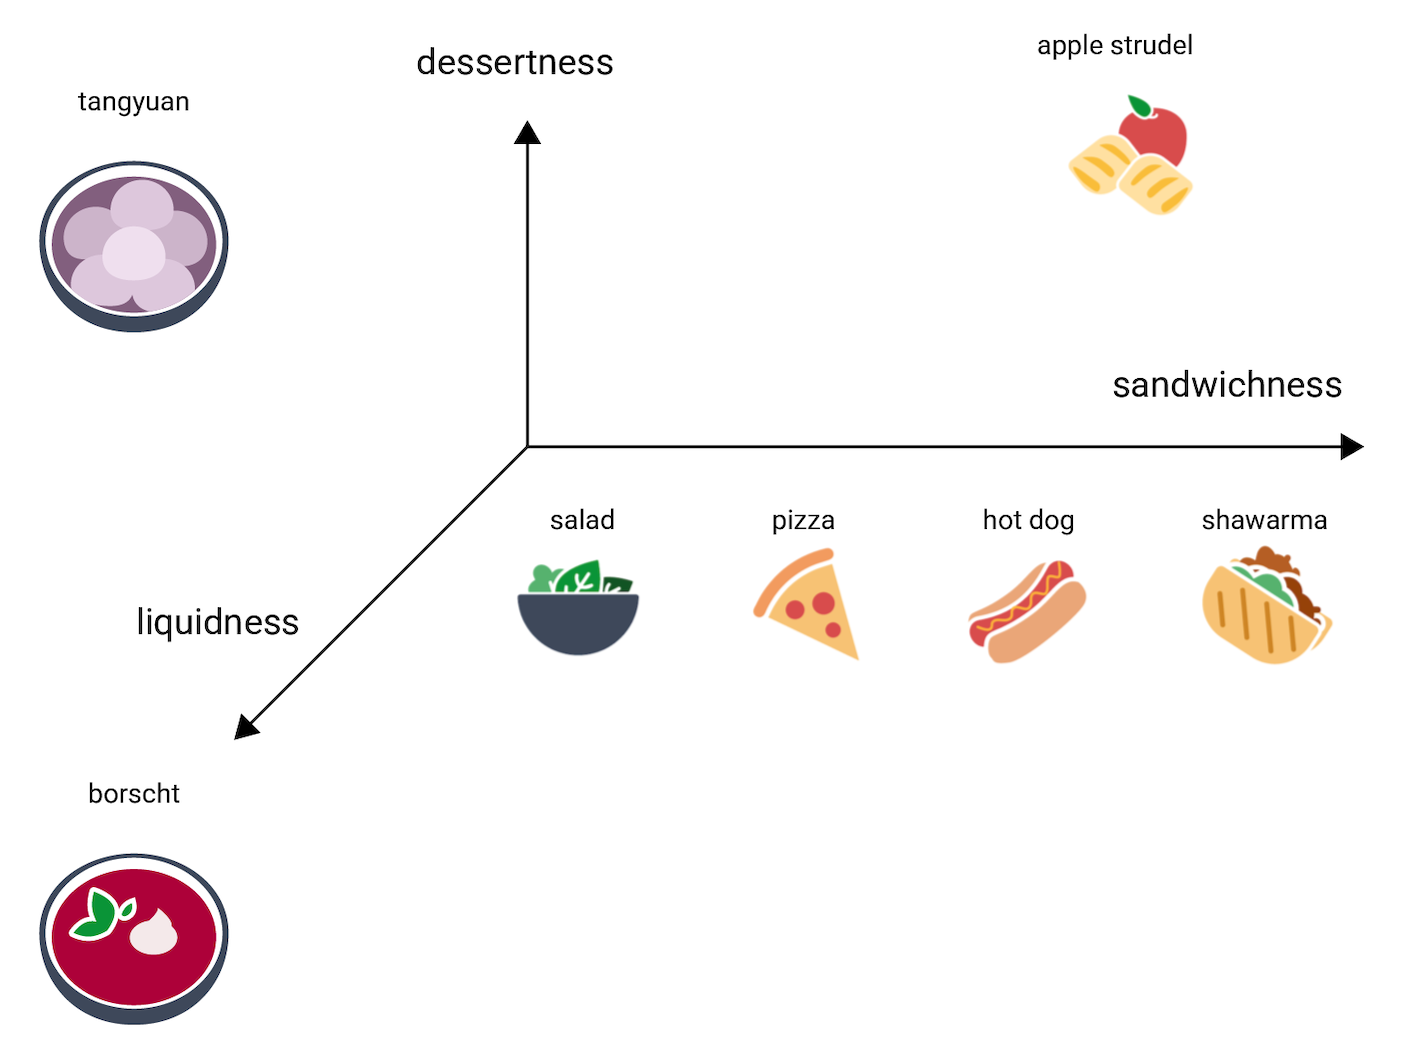
\includegraphics[height=4.6cm]{embeddings_3D_tangyuan.png}\\[1pt]
{\scriptsize\itshape Con comidas bastan 3 preguntas. Con texto es igual, pero con \textbf{cientos}.}\\[1pt]
{\tiny\color{uaigray} Imagen de Google, \textit{ML Crash Course} (CC BY 4.0).}
\end{column}

\end{columns}

\mensaje{Con los textos convertidos en puntos, «parecerse» se vuelve algo que podemos \emph{medir}.}
\end{frame}

% --- Slide: Intro SMOTE (simplificada para divulgación; fórmula fuera) ---
\begin{frame}{Camino 1 — SMOTE: inventar puntos intermedios en el mapa}
\begin{columns}[T]

\begin{column}{0.55\textwidth}
\small
\textbf{SMOTE} \cita{Chawla et al., 2002} es el método clásico (20+ años) para crear ejemplos de la clase escasa.

\vspace{0.4em}
\textbf{La idea, en una frase:}
\begin{itemize}\setlength\itemsep{2pt}
  \item Toma dos ejemplos reales que sean vecinos en el mapa\dots
  \item \dots{}y crea un punto nuevo \alert{en el camino entre ambos}: un «promedio» de los dos.
\end{itemize}

\vspace{0.6em}
\good\ Controlado: nunca se sale de la zona conocida.\\
\good\ Simple y rápido; funciona hace décadas.\\[3pt]
\bad\ Genera \alert{puntos, no texto}: no hay oración nueva que leer.\\
\bad\ Solo \alert{rellena} lo que ya se sabe: no aporta variedad nueva.
\end{column}

\begin{column}{0.45\textwidth}
\centering
\vspace{0.3em}
\begin{tikzpicture}[scale=1.0]
  % Casco convexo
  \fill[methodSMOTE!10] (-1.3,-1.1) -- (1.3,-0.9) -- (1.5,0.7) -- (-0.5,1.3) -- (-1.3,-1.1);

  % Puntos reales
  \foreach \pt in {(-1.3,-1.1),(1.3,-0.9),(1.5,0.7),(-0.5,1.3),(0,0.2)}{\fill[methodSMOTE] \pt circle (3.5pt);}

  % Segmentos de interpolación
  \draw[methodSMOTE!60, dashed] (-1.3,-1.1) -- (1.3,-0.9);
  \draw[methodSMOTE!60, dashed] (-1.3,-1.1) -- (0,0.2);
  \draw[methodSMOTE!60, dashed] (0,0.2) -- (1.5,0.7);
  \draw[methodSMOTE!60, dashed] (-0.5,1.3) -- (0,0.2);

  % Sintéticos (en los segmentos)
  \foreach \pt in {(0,-1),(-0.65,-0.45),(0.75,0.45),(-0.25,0.75)}{\draw[uaiorange, very thick] \pt circle (3pt);}

  \node[font=\tiny, color=uaigray] at (0,-1.8) {{\color{methodSMOTE}\textbullet}\,reales \quad {\color{uaiorange}$\circ$}\,inventados};
  \node[font=\tiny\itshape] at (0,-2.1) {Puntos nuevos entre vecinos};
\end{tikzpicture}
\end{column}

\end{columns}

\mensaje{Control total sobre dónde caen los puntos\dots\ pero sin texto nuevo y sin nada realmente nuevo.}
\end{frame}

% =============================================================================
% [DIVULGACIÓN] Slide comentada para la versión de público general.
% Reactivar quitando \iffalse ... \fi si se necesita de nuevo (versión defensa).
% =============================================================================
\iffalse
% --- Slide: Familia 2 — Aumentación textual ligera (entre SMOTE y LLMs) ---
\begin{frame}{Familia 2 — Aumentación textual ligera}
\small
Entre la \alert{interpolación geométrica} y la \alert{generación libre} hay un puente histórico: métodos que producen texto con modelos pequeños y operaciones controladas.

\vspace{0.5em}
\begin{columns}[T]

\begin{column}{0.33\textwidth}
\setbeamercolor{block title}{fg=white,bg=uaiblue}
\begin{block}{EDA}
\scriptsize
\cita{Wei \& Zou, 2019}\\[3pt]
4 ops a nivel \textbf{palabra}:\\
sinónimo, inserción, swap, deleción.\\[3pt]
\good\ Muy barato.\\
\bad\ Ruido en oraciones cortas.
\end{block}
\end{column}

\begin{column}{0.33\textwidth}
\setbeamercolor{block title}{fg=white,bg=uaiblue}
\begin{block}{Traducción inversa}
\scriptsize
\cita{Sennrich 2016; Edunov 2018}\\[3pt]
EN $\to$ otro idioma $\to$ EN.\\
Paráfrasis a nivel \textbf{oración}.\\[3pt]
\good\ Cambia sintaxis.\\
\bad\ Pierde matices.
\end{block}
\end{column}

\begin{column}{0.33\textwidth}
\setbeamercolor{block title}{fg=white,bg=uaiblue}
\begin{block}{BERT contextual}
\scriptsize
\cita{Kobayashi 2018; Wu 2019}\\[3pt]
Enmascarar tokens; BERT predice alternativas plausibles.\\[3pt]
\good\ Contexto semántico.\\
\bad\ Solo sustitución 1:1.
\end{block}
\end{column}

\end{columns}

\vspace{0.7em}
\begin{insight}
\scriptsize
Todos producen \textbf{texto}, pero con un \textbf{techo de creatividad bajo}: paráfrasis cercanas al original. Los LLMs rompen ese techo --- y por eso necesitan otro tipo de control.
\end{insight}
\end{frame}
\fi

% --- Slide: Camino 2 — LLMs ---
\begin{frame}{Camino 2 — Pedirle los ejemplos a una IA (LLM)}
\begin{columns}[T]

\begin{column}{0.58\textwidth}
\small
Pedirle a una IA generativa (ChatGPT, Gemini, Claude\dots) que \textbf{escriba ejemplos nuevos} para la clase que tiene pocos.

\vspace{0.4em}
\textbf{La receta que se usa hoy:}
\begin{enumerate}\setlength\itemsep{2pt}\small
  \item Mostrarle los pocos ejemplos reales que hay.
  \item Pedirle: «escribe 50 más como estos».
  \item Agregar \textbf{todo} lo que responda al entrenamiento.
\end{enumerate}

\vspace{0.4em}
Varios estudios reportan mejoras \cita{Whitehouse 2023; Suhaeni 2024; Cegin 2025} — pero todos comparten el mismo punto ciego.

\vspace{0.4em}
{\small
\good\ Texto real, fluido y variado.\\
\bad\ \alert{Nadie revisa dónde caen} esos textos en el mapa: se acepta todo, bueno y malo.}
\end{column}

\begin{column}{0.42\textwidth}
\centering
\vspace{0.2em}
\begin{tikzpicture}[every node/.style={font=\scriptsize, align=center}]
  \node[draw=uaibluedark, fill=uaibluelight!15, rounded corners, very thick,
        text width=3.6cm, minimum height=1.0cm] (prompt) at (0, 2.7)
        {\scriptsize\textbf{Prompt}\\[1pt]
         \tiny\itshape ``Genera 50 mensajes de alegría\dots''};
  \draw[->, very thick, uaibluedark] (0, 2.05) -- (0, 1.65);
  \node[draw=methodOurs, fill=methodOurs!15, rounded corners, very thick,
        text width=2.4cm, minimum height=0.7cm] (llm) at (0, 1.2)
        {\textbf{LLM}};
  \draw[->, very thick, methodOurs] (0, 0.8) -- (0, 0.4);
  \node[draw=uaiorange, fill=uaiorange!10, rounded corners, very thick,
        text width=3.6cm, minimum height=1.0cm] (out) at (0, -0.2)
        {\scriptsize\textbf{$N$ oraciones nuevas}\\[1pt]
         \tiny algunas buenas, otras ruido\dots};
\end{tikzpicture}
\end{column}

\end{columns}

\mensaje{Texto rico pero sin control: los puntos caen donde quieran en el mapa.}
\end{frame}

% =============================================================================
% [DIVULGACIÓN] Slide comentada para la versión de público general.
% Reactivar quitando \iffalse ... \fi si se necesita de nuevo (versión defensa).
% =============================================================================
\iffalse
% --- Slide: Familia 3.5 — Fine-tuning para generación sintética ---
\begin{frame}{Familia 3.5 — \textit{Fine-tuning} para generación sintética}
\begin{columns}[T]

\begin{column}{0.58\textwidth}
\small
Una rama más reciente: \alert{ajustar el LLM} sobre la propia tarea antes de generar.

\vspace{0.2em}
\textbf{Idea:} fine-tunear un LLM preentrenado (GPT-2, LLaMA, T5\dots) con los pocos ejemplos disponibles, y luego generar muestras \emph{específicas} del dominio.

\vspace{0.3em}
\textbf{Trabajos representativos:}
\begin{itemize}\setlength\itemsep{0pt}\scriptsize
  \item Cloutier \& Japkowicz (2023): \alert{fine-tuning generativo} supera al re-muestreo tradicional en multiclase desbalanceada.
  \item ImbLLM (Nguyen et al., 2024): fine-tuning \textbf{solo en muestras minoritarias}; F1\,$>$\,0.8.
  \item SentiGEN (Sundararajan, 2023): T5 fine-tuned + validador XLNet.
\end{itemize}

\vspace{0.3em}
{\scriptsize
\good\ Distribución alineada con la tarea.\\
\bad\ Requiere \alert{cómputo extra}; riesgo de \emph{overfitting} con $n$ pequeño.}
\end{column}

\begin{column}{0.42\textwidth}
\centering
\vspace{0.1em}
\begin{tikzpicture}[every node/.style={font=\scriptsize, align=center}, scale=0.92, transform shape]
  % LLM base
  \node[draw=uaibluedark, fill=uaibluelight!15, rounded corners, very thick,
        text width=3.0cm, minimum height=0.55cm] (base) at (0, 2.6)
        {\textbf{LLM preentrenado}\\\tiny GPT-2, LLaMA, T5\dots};

  % Few-shot data
  \node[draw=methodSMOTE, fill=methodSMOTE!15, rounded corners, very thick,
        text width=1.9cm, minimum height=0.45cm, font=\scriptsize] (data) at (-1.95, 1.55)
        {Pocos ej.};

  % Fine-tune arrow
  \node[draw=uaiamber, fill=uaiamber!15, rounded corners, very thick,
        text width=1.7cm, minimum height=0.45cm, font=\scriptsize\bfseries] (ft) at (0.6, 1.55)
        {Fine-tuning};
  \draw[->, very thick, uaiamber] (data) -- (ft);
  \draw[->, very thick, uaiamber] (base) -- (ft);

  % LLM ajustado
  \node[draw=methodOurs, fill=methodOurs!15, rounded corners, very thick,
        text width=3.0cm, minimum height=0.55cm] (llmft) at (0, 0.55)
        {\textbf{LLM ajustado}\\\tiny especializado};
  \draw[->, very thick, methodOurs] (ft) -- (llmft);

  % Output
  \node[draw=uaiorange, fill=uaiorange!10, rounded corners, very thick,
        text width=3.0cm, minimum height=0.5cm] (out) at (0, -0.45)
        {\scriptsize\textbf{Muestras sintéticas}\\\tiny alineadas al dominio};
  \draw[->, very thick, uaiorange] (llmft) -- (out);
\end{tikzpicture}
\end{column}

\end{columns}

\mensaje{Más alineamiento, más costo: distinto eje de control al filtrado posterior.}
\end{frame}
\fi

% --- Slide: El dilema (movido desde Introducción) ---
\begin{frame}{El dilema: SMOTE vs.\ LLMs lado a lado}
\begin{columns}[T]

\begin{column}{0.5\textwidth}
\centering
\setbeamercolor{block title}{fg=white,bg=methodSMOTE}
\begin{block}{SMOTE / interpolación}
\small
\good\ Sabemos \textbf{dónde} caen sus puntos\\
\good\ Probado por más de 20 años\\[2pt]
\bad\ No produce texto nuevo\\
\bad\ Solo rellena lo ya conocido
\end{block}
\vspace{0.2em}
\begin{tikzpicture}[scale=0.85]
  \fill[methodSMOTE!20] (0,0) circle (1.4);
  \foreach \pt in {(0,0.4),(0.7,0.2),(-0.5,0.6),(0.3,-0.5),(-0.7,-0.3),(0.6,-0.7)} {\fill[methodSMOTE] \pt circle (2pt);}
  \foreach \pt in {(0.4,0),(-0.2,0.1),(0.1,0.5),(-0.4,-0.5),(0.45,-0.2)} {\draw[uaiorange,thick] \pt circle (2pt);}
  \node[font=\tiny] at (0,-1.7) {Todo queda dentro de la zona conocida};
\end{tikzpicture}
\end{column}

\begin{column}{0.5\textwidth}
\centering
\setbeamercolor{block title}{fg=white,bg=methodOurs}
\begin{block}{LLM (Gemini, GPT, Claude\dots)}
\small
\good\ Texto fluido y variado\\
\good\ Aporta contenido \textbf{nuevo}\\[2pt]
\bad\ No sabemos dónde caen sus puntos\\
\bad\ Puede mezclar clases (ruido)
\end{block}
\vspace{0.4em}
\begin{tikzpicture}[scale=0.85]
  \fill[methodOurs!15] (0,0) circle (1.6);
  \foreach \pt in {(0,0.4),(0.7,0.2),(-0.5,0.6),(0.3,-0.5)} {\fill[methodOurs] \pt circle (2pt);}
  \foreach \pt in {(0.4,0),(-0.2,0.1),(0.1,0.5),(1.4,0.3),(-1.2,-0.4),(0.9,-1.0),(-0.8,1.1)} {\draw[uaiorange,thick] \pt circle (2pt);}
  \node[font=\tiny] at (0,-1.9) {Los puntos caen donde sea};
\end{tikzpicture}
\end{column}

\end{columns}

\mensaje{¿Podemos quedarnos con lo mejor de ambos mundos?}
\end{frame}

% =============================================================================
% [DIVULGACIÓN] Slide comentada para la versión de público general.
% Reactivar quitando \iffalse ... \fi.
% =============================================================================
\iffalse
% --- Slide: Tres deficiencias (después del Timeline) ---
\begin{frame}{Tres deficiencias en los métodos actuales}
\small
\begin{columns}[T]

\begin{column}{0.33\textwidth}
\setbeamercolor{block title}{fg=white,bg=uaiorange}
\begin{block}{1. Sin control de calidad}
Lo que escribe la IA se acepta \textbf{todo}, sin revisar si cada texto cayó en la zona correcta del mapa.
\vspace{0.3em}\\
{\scriptsize Que esté bien escrito $\neq$ que sea un buen ejemplo.}
\end{block}
\end{column}

\begin{column}{0.33\textwidth}
\setbeamercolor{block title}{fg=white,bg=uaiamber}
\begin{block}{2. Todo pesa igual}
Al entrenar, un ejemplo dudoso cuenta \textbf{lo mismo} que uno excelente.
\vspace{0.3em}\\
{\scriptsize Nadie distingue entre buenos y mediocres.}
\end{block}
\end{column}

\begin{column}{0.33\textwidth}
\setbeamercolor{block title}{fg=white,bg=uaiblue}
\begin{block}{3. Poca evidencia}
Casi todos los estudios prueban su método en \textbf{un solo} conjunto de datos.
\vspace{0.3em}\\
{\scriptsize ¿Funcionará también en otros temas y tareas?}
\end{block}
\end{column}

\end{columns}

\vfill
\begin{tikzpicture}[overlay,remember picture]
\end{tikzpicture}

\mensaje{El mapa ya existe y nadie lo está usando para controlar la calidad.}
\end{frame}
\fi

% --- Slide: Gap metodológico + idea conceptual ---
\begin{frame}{La idea de esta tesis: ponerle un control de calidad a la IA}
\begin{columns}[T]

\begin{column}{0.52\textwidth}
\small
Nadie revisa dónde caen los textos que escribe la IA. Eso abre una solución sorprendentemente simple.

\vspace{0.2em}
\textbf{La idea:}
\begin{enumerate}\setlength\itemsep{1pt}\footnotesize
  \item Pedirle a la IA \textbf{más ejemplos de los necesarios}.
  \item Ubicar cada uno como un punto en el mapa.
  \item Medir qué tan cerca cae de los \textbf{ejemplos reales} de su clase.
  \item \alert{Descartar los que caen demasiado lejos}.
\end{enumerate}

\vspace{0.3em}
\textbf{¿Por qué tiene sentido?}
\begin{itemize}\setlength\itemsep{1pt}\footnotesize
  \item El mapa \alert{ya lo teníamos}: es el mismo que usa el clasificador.
  \item Sirve cualquier IA (Gemini, GPT, Claude\dots): no hay que abrirla ni re-entrenarla.
\end{itemize}
\end{column}

\begin{column}{0.48\textwidth}
\centering
\vspace{0.2em}
\begin{tikzpicture}[scale=0.85]
  % Cluster real (fondo)
  \fill[methodSMOTE!18] (0,0) circle (1.5);

  % Frontera del filtro (dashed)
  \draw[uaibluedark, dashed, thick] (0,0) circle (1.9);

  % Puntos reales (sólidos)
  \foreach \pt in {(0,0.2),(0.4,0.4),(-0.5,0.3),(0.6,-0.4),(-0.3,-0.5),(0.2,0.7),(-0.6,-0.2),(0.7,0.1)} {\fill[methodSMOTE] \pt circle (3pt);}

  % LLM aceptados (verdes, dentro del filtro)
  \foreach \pt in {(0.9,0.5),(-0.8,-0.7),(0.3,1.0),(-0.4,1.1),(1.0,-0.5),(-1.1,0.4)} {\draw[methodOurs, very thick] \pt circle (3pt);}

  % LLM rechazados (rojos, fuera del filtro)
  \foreach \pt in {(2.4,0.7),(-2.3,0.9),(2.0,-1.4),(-1.7,-2.0),(0.1,2.3),(2.5,-0.3)} {\draw[uaiorange, very thick] \pt circle (3pt);}

  % Leyenda compacta
  \node[font=\tiny, color=methodSMOTE, anchor=west] at (-2.8,3.0) {{\fontsize{6}{6}\selectfont$\bullet$}\,reales};
  \node[font=\tiny, color=methodOurs, anchor=west] at (-2.8,2.7) {$\circ$\,aceptado};
  \node[font=\tiny, color=uaiorange, anchor=west] at (-2.8,2.4) {$\circ$\,rechazado};
  \node[font=\tiny, color=uaibluedark, anchor=west] at (-2.8,2.1) {- -\,filtro};
\end{tikzpicture}
\end{column}

\end{columns}

\mensaje{Lo mejor de ambos mundos: el texto lo pone la IA, el control de calidad lo pone el mapa.}
\end{frame}



% --- Bloque 5: Hipótesis y Objetivos ---
% =============================================================================
% Bloque 5: Hipótesis y Objetivos (slide 11)
% =============================================================================

\section{Hipótesis y objetivos}

% --- Slide 11: H1 + objetivo general + sub-hipótesis + específicos ---
\begin{frame}[c]{Hipótesis y objetivos}
\setbeamercolor{block title}{fg=white,bg=uaiorange}
\begin{block}{H1 — Hipótesis principal}
\small
Si a los ejemplos que escribe la IA les aplicamos un \textbf{control de calidad en el mapa}
(quedarnos con los bien ubicados), el clasificador mejora \textbf{más que con SMOTE},
el método clásico — y la mejora es real, \textbf{no producto del azar}.
\end{block}

\setbeamercolor{block title}{fg=white,bg=uaibluedark}
\begin{block}{Objetivo general}
\small
Desarrollar y validar ese control de calidad de modo que funcione \textbf{mirando solo el mapa}:
sin importar qué IA escribió el texto, y en escenarios con \textbf{pocos ejemplos por clase}.
\end{block}

\end{frame}


% --- Bloque 6: Metodología ---
% =============================================================================
% Bloque 6: Metodología (slides 12–16)
% =============================================================================

\section{Metodología}

% --- Slide 12: Pipeline arquitectónico ---
\begin{frame}{Pipeline: del texto real al clasificador entrenado}
\centering
\begin{tikzpicture}[
    every node/.style={font=\scriptsize},
    box/.style={draw=uaiblue, rounded corners, fill=uaibluelight!15,
                minimum width=2cm, minimum height=0.9cm, text width=2cm, align=center},
    box2/.style={draw=uaiorange, very thick, rounded corners, fill=uaiorange!15,
                 minimum width=2cm, minimum height=0.9cm, text width=2cm, align=center},
    box3/.style={draw=uaigreen, very thick, rounded corners, fill=uaigreen!15,
                 minimum width=2cm, minimum height=0.9cm, text width=2cm, align=center},
    arrow/.style={->, >=Stealth, thick, uaiblue!70}
  ]
  % Fila superior
  \node[box]  (real)  at (0,2)    {\textbf{Datos\\reales}\\\tiny 10/25/50 por clase};
  \node[box]  (enc)   at (2.6,2)  {\textbf{Al mapa}\\\tiny embeddings};
  \node[box]  (llm)   at (5.2,2)  {\textbf{IA genera}\\\tiny Gemini\\\tiny $3\times$ de sobra};
  \node[box]  (cands) at (7.8,2)  {\textbf{Candidatas}\\\tiny puntos en el mapa};
  \node[box2] (filt)  at (10.4,2) {\textbf{Control de calidad}\\\tiny filtro geométrico};

  % Fila inferior
  \node[box2] (weight) at (10.4,0)  {\textbf{Pesos}\\\tiny según calidad};
  \node[box3] (clf)    at (5.2,0)   {\textbf{Clasificador}\\\tiny 5 tipos distintos};
  \node[box]  (eval)   at (0,0)     {\textbf{Evaluación}\\\tiny con datos nunca vistos};

  % Flechas
  \draw[arrow] (real)  -- (enc);
  \draw[arrow] (enc)   -- (llm);
  \draw[arrow] (llm)   -- (cands);
  \draw[arrow] (cands) -- (filt);
  \draw[arrow] (filt)  -- (weight);
  \draw[arrow] (weight) -- (clf);
  \draw[arrow] (real.south)  .. controls +(0,-0.6) and +(-0.5,0) .. (clf.west);
  \draw[arrow] (clf)   -- (eval);
  % Atajo punteado: filtro binario (sin ponderación suave)
  \draw[->, >=Stealth, thick, uaibluedark!60, dashed]
       (filt.south west) .. controls +(-1.2,-0.7) and +(1.0,0.7) ..
       node[midway, above, font=\tiny\itshape, color=uaibluedark!70] {sin pesos}
       (clf.north east);
\end{tikzpicture}

\vspace{0.5em}
\mensaje{Las dos piezas nuevas (control de calidad y pesos) no tocan la IA: funcionan con cualquiera.}
\end{frame}

% --- Slide 13: Protocolo experimental (vuelve, antes de los datasets) ---
\begin{frame}{Protocolo experimental: 8.000+ experimentos}
\small
\begin{columns}[T]

\begin{column}{0.55\textwidth}
\textbf{Probamos la idea en todas las combinaciones:}
\begin{itemize}\setlength\itemsep{0pt}
  \item \textbf{13 conjuntos de datos} en 9 dominios.
  \item \textbf{Escasez:} 10 / 25 / 50 ejemplos por clase.
  \item \textbf{5 tipos} de clasificador.
  \item \textbf{10 métodos} de aumentación en competencia.
  \item \textbf{5 IAs generadoras} (Gemini, GPT-5, Claude, Kimi, GLM).
  \item \textbf{4 mapas} (modelos de embeddings) distintos.
  \item \textbf{5 repeticiones} de cada experimento.
\end{itemize}
\end{column}

\begin{column}{0.45\textwidth}
\textbf{Cómo comparamos:}
\begin{itemize}\setlength\itemsep{0pt}
  \item Nota de calidad: \textbf{macro F1} (siguiente slide).
  \item Cada método compite contra \textbf{SMOTE} en el mismo escenario exacto.
  \item Pruebas estadísticas estrictas: descartan que la diferencia sea \alert{azar}.
  \item También contamos \textbf{cuántas veces gana} cada método.
\end{itemize}

\vspace{0.3em}
\setbeamercolor{block title}{fg=white,bg=uaiorange}
\begin{block}{Volumen}
\centering\bfseries\large 8.000+ experimentos
\end{block}
\end{column}

\end{columns}
\end{frame}

% --- Slide 13b: Métrica de evaluación — Macro F1 (sin fórmulas, versión divulgación) ---
\begin{frame}{¿Cómo medimos el éxito? Una nota justa: macro F1}
\begin{columns}[T]

\begin{column}{0.55\textwidth}
\small
\textbf{El acierto global engaña:} un modelo que responde siempre «clase común» acierta el 95\%\dots\ ignorando por completo a la clase rara.

\vspace{0.5em}
\textbf{Macro F1} hace algo más justo:
\begin{enumerate}\setlength\itemsep{3pt}
  \item Le pone una \textbf{nota de 0 a 100 a cada clase}: qué tan bien la detecta, sin confundirla con otras.
  \item \textbf{Promedia las notas}: cada clase pesa lo mismo, tenga 16 ejemplos o 720.
\end{enumerate}

\vspace{0.5em}
\begin{insight}
\scriptsize
Como el promedio de notas por ramo: sacarse un 7 en el ramo fácil \textbf{no tapa} el 2 en el difícil.
\end{insight}
\end{column}

\begin{column}{0.45\textwidth}
\setbeamercolor{block title}{fg=white,bg=uaiblue}
\begin{block}{\small Por qué nos sirve}
\scriptsize
\begin{itemize}\setlength\itemsep{1pt}
  \item Un error en la clase rara \textbf{duele igual} que uno en la clase grande.
  \item Si el modelo \emph{ignora} una clase chica, la nota cae de inmediato.
\end{itemize}
\end{block}

\vspace{0.4em}
\setbeamercolor{block title}{fg=white,bg=uaiorange}
\begin{block}{\small Cómo leerán los resultados}
\scriptsize
\begin{itemize}\setlength\itemsep{1pt}
  \item $\Delta$F1 $=$ cuántos \textbf{puntos de nota} sube (o baja) un método frente a SMOTE.
  \item «pp» $=$ puntos porcentuales: $+2$ pp $=$ subir de 71 a 73.
  \item Siempre evaluado sobre datos que el modelo \textbf{nunca vio}.
\end{itemize}
\end{block}
\end{column}

\end{columns}

\mensaje{Macro F1: la métrica honesta cuando hay clases raras.}
\end{frame}

% --- Slide 14: Conjuntos de datos (tabla) ---
\begin{frame}{Conjuntos de datos: 13 corpus en 9 dominios}
\centering
\scriptsize
\renewcommand{\arraystretch}{0.92}
\begin{tabular}{@{}llccr@{}}
\toprule
\textbf{Conjunto} & \textbf{Dominio} & \textbf{Clases} & \textbf{$n$-shots} & \textbf{Test} \\
\midrule
\rowcolor{uaibluelight!12}\multicolumn{5}{l}{\textit{\color{uaibluedark}Clasificación de texto --- experimento principal}} \\
\dataset{sms\_spam}              & Detección de spam        & 2  & 10, 25, 50 & 1.394 \\
\dataset{hate\_speech\_davidson} & Discurso de odio         & 3  & 10, 25, 50 & 4.948 \\
\dataset{20newsgroups}           & Noticias (4 cat.)        & 4  & 10, 25, 50 & 7.532 \\
\dataset{ag\_news}               & Noticias (4 cat.)        & 4  & 10, 25, 50 & 7.600 \\
\dataset{emotion}                & Emociones                & 6  & 10, 25, 50 & 2.000 \\
\dataset{dbpedia14}              & Clasificación de temas   & 14 & 10, 25, 50 & 5.000 \\
\dataset{20newsgroups\_20class}  & Noticias (20 cat.)       & 20 & 10, 25, 50 & 7.532 \\
\midrule
\rowcolor{uaiorange!12}\multicolumn{5}{l}{\textit{\color{uaibluedark}Adicionales --- escalabilidad por número de clases}} \\
\dataset{trec6}                  & Preguntas                & 6   & 10, 25, 50 & 500 \\
\dataset{banking77}              & Intenciones bancarias    & 77  & 10, 25, 50 & 3.080 \\
\dataset{clinc150}               & Intenciones de diálogo   & 150 & 10, 25, 50 & 4.500 \\
\midrule
\rowcolor{uaigreen!12}\multicolumn{5}{l}{\textit{\color{uaibluedark}Reconocimiento de entidades nombradas (NER)}} \\
\dataset{MultiNERD}              & Entidades generales      & 5 tipos & 10, 25, 50 & 10.000 \\
\dataset{WikiANN}                & Entidades Wikipedia      & 3 tipos & 10, 25, 50 & 10.000 \\
\dataset{Few-NERD}               & Entidades detalladas     & 8 tipos & 10, 25, 50 & 10.000 \\
\bottomrule
\end{tabular}

\vspace{0.2em}
{\scriptsize\itshape $n$-shot estricto: 10 / 25 / 50 ejemplos por clase. Rango de complejidad: de binario (\dataset{sms\_spam}) a 150 clases (\dataset{clinc150}).}
\end{frame}

% --- Slide 16: ¿Qué es NER y por qué la usamos? ---
\begin{frame}{¿Qué es NER y por qué la usamos?}

\setbeamercolor{block title}{fg=white,bg=uaibluedark}
\begin{block}{\small NER (\textit{Named Entity Recognition})}
\scriptsize
Tarea de NLP que \textbf{detecta nombres propios dentro del texto y los clasifica por tipo}: personas, lugares, organizaciones, fechas, etc.

\vspace{0.3em}
\textit{Ejemplo:} «Llamé a \colorbox{uaiblue!25}{\strut\,María\,} en \colorbox{uaiorange!25}{\strut\,Madrid\,} el \colorbox{uaigreen!25}{\strut\,2 de marzo\,}.»\hspace{0.5em}{\tiny \textcolor{uaiblue}{$\uparrow$PER}\hspace{1em}\textcolor{uaiorange}{$\uparrow$LOC}\hspace{1em}\textcolor{uaigreen}{$\uparrow$DATE}}
\end{block}

\vspace{0.4em}
\begin{columns}[T]

\begin{column}{0.55\textwidth}
\small
\textbf{¿Por qué la usamos como prueba?}
\begin{itemize}\setlength\itemsep{1pt}\scriptsize
  \item Construimos el filtro para \textbf{clasificación}.
  \item NER es una tarea NLP \textbf{distinta}: en vez de etiquetar la oración entera, se etiquetan palabras dentro.
  \item Si el mismo filtro funciona en NER \textbf{sin cambiarlo} $\Rightarrow$ el filtro \alert{no depende de la tarea}.
\end{itemize}

\vspace{0.2em}
{\scriptsize Es la prueba más fuerte de que el método \textbf{generaliza}.}
\end{column}

\begin{column}{0.45\textwidth}
\setbeamercolor{block title}{fg=white,bg=uaigreen}
\begin{block}{\small 3 corpus, distinta complejidad}
\scriptsize
\begin{itemize}\setlength\itemsep{1pt}
  \item \dataset{WikiANN} --- 3 tipos (PER, ORG, LOC). \textbf{Fácil}.
  \item \dataset{MultiNERD} --- 5 tipos (+ DATE, MISC). Medio.
  \item \dataset{Few-NERD} --- 8 tipos jerárquicos. \textbf{Difícil}.
\end{itemize}
\end{block}
\end{column}

\end{columns}

\mensaje{Mismo filtro, otra tarea: si funciona acá, sirve en general.}
\end{frame}

% --- Slide 17: Los 4 filtros (versión divulgación) ---
\begin{frame}{Cuatro maneras de hacer el control de calidad}
\small
Probamos cuatro «porteros» distintos, del más permisivo al más estricto:

\vspace{0.5em}
\begin{tabular}{@{}p{2.9cm}p{9.2cm}@{}}
\toprule
\textbf{Filtro} & \textbf{La pregunta que le hace a cada candidata} \\
\midrule
\textit{Ninguno} (control)  & Deja pasar todo. Sirve de punto de comparación. \\[4pt]
\textit{LOF} (densidad)     & ¿Caíste en una zona \textbf{poblada} de tu clase, o en un descampado? \\[4pt]
\textit{Cascada} (niveles 1--4) & ¿Qué tan \textbf{cerca} caíste de los ejemplos reales? Ordena a todas las candidatas y se queda con las mejores. \\[4pt]
\textit{Combinado}          & Exige \textbf{dos condiciones a la vez} (densidad \textbf{y} parecido). El portero más estricto. \\
\bottomrule
\end{tabular}

\mensaje{Mismo mapa, cuatro criterios: ¿cuál elige mejor?}
\end{frame}

% --- Slide 14: Cascade — pieza central (versión divulgación, sin fórmulas) ---
\begin{frame}{La cascada: cuatro preguntas sobre cada candidata}
\begin{columns}[T]

\begin{column}{0.55\textwidth}
\small
Cada texto que escribe la IA recibe un \textbf{puntaje de calidad} según dónde cayó su punto en el mapa. Cuatro preguntas, de la más simple a la más elaborada:

\vspace{0.4em}
\begin{description}\setlength\itemsep{4pt}\small
  \item[Nivel 1 \alert{$\star$}] \textbf{Cercanía:} ¿qué tan cerca caíste del ejemplo real más próximo?
  \item[Nivel 2] \textbf{Parecido:} ¿te «pareces» a ese ejemplo? (similitud de significado)
  \item[Nivel 3] \textbf{Vecindario:} ¿tus vecinos en el mapa son de tu misma clase?
  \item[Nivel 4] \textbf{Centro:} ¿qué tan cerca estás del centro de tu clase?
\end{description}

\vspace{0.4em}
Las preguntas activas se combinan en un solo puntaje, y nos quedamos con las \textbf{$N$ mejores} candidatas del ranking.
\end{column}

\begin{column}{0.45\textwidth}
\centering
\begin{tikzpicture}[every node/.style={font=\tiny}]
  % Pirámide de niveles
  \fill[uaiorange!40] (-2.5,2.4) rectangle (2.5,3.0);
  \node[font=\scriptsize\bfseries] at (0,2.7) {Nivel 1: Cercanía $\star$};

  \fill[uaibluelight!30] (-2.2,1.7) rectangle (2.2,2.3);
  \node[font=\scriptsize] at (0,2.0) {Nivel 2: Parecido};

  \fill[uaibluelight!20] (-1.9,1.0) rectangle (1.9,1.6);
  \node[font=\scriptsize] at (0,1.3) {Nivel 3: Vecindario};

  \fill[uaibluelight!15] (-1.6,0.3) rectangle (1.6,0.9);
  \node[font=\scriptsize] at (0,0.6) {Nivel 4: Centro de clase};

  % Flecha de score
  \draw[->, very thick, uaiorange] (-3.2,0.3) -- (-3.2,3.0);
  \node[font=\tiny, rotate=90] at (-3.6,1.65) {puntaje $\uparrow$};
\end{tikzpicture}\\[4pt]
{\scriptsize Se queda con las \textbf{$N$ mejores} del ranking\\ (no hay nota mínima de corte).}

\vspace{0.5em}
\begin{insight}
\scriptsize \textbf{Adelanto:} la pregunta más simple —el Nivel 1, pura cercanía— resultará ser la única necesaria.
\end{insight}
\end{column}

\end{columns}
\end{frame}

% --- Slide 15: Ponderación suave (versión divulgación, sin ecuaciones) ---
\begin{frame}{Ponderación suave: no todas las muestras valen lo mismo}
\begin{columns}[T]

\begin{column}{0.5\textwidth}
\small
La segunda contribución: en vez de \textbf{aceptar o rechazar} en seco, cada muestra entra al entrenamiento con un \textbf{peso según su puntaje}.

\vspace{0.4em}
\begin{itemize}\setlength\itemsep{2pt}
  \item \textbf{Ejemplo real} $\Rightarrow$ peso máximo (1): en ellos confiamos siempre.
  \item \textbf{Candidata bien ubicada} $\Rightarrow$ peso alto.
  \item \textbf{Candidata dudosa} $\Rightarrow$ peso bajo: se usa, pero \alert{se le cree menos}.
\end{itemize}

\vspace{0.4em}
\begin{insight}
\scriptsize
Como un profesor que escucha a todo el curso, pero pondera más las respuestas de quienes muestran su desarrollo.
\end{insight}
\end{column}

\begin{column}{0.5\textwidth}
\centering
\begin{tikzpicture}[every node/.style={font=\tiny}]
  % Eje
  \draw[->,uaigray] (0,0) -- (4.5,0) node[right]{puntaje};
  \draw[->,uaigray] (0,0) -- (0,3.2) node[above]{peso};
  \node[font=\tiny] at (4,-0.25) {1};
  \node[font=\tiny] at (-0.2,3) {1};

  % Curva tau=0.5 (peaked) — w = s^2
  \draw[very thick, uaiorange, domain=0:4, samples=40, smooth] plot (\x, {3*(\x/4)^2});
  \node[uaiorange, font=\scriptsize, align=center] at (3.1,2.75) {curva exigente\\(la que usamos)};

  % Curva tau=1 (linear)
  \draw[thick, uaiblue, dashed, domain=0:4, samples=40] plot (\x, {3*(\x/4)});
  \node[uaiblue, font=\scriptsize, align=center] at (3.7,1.35) {curva\\neutra};

  \node[align=center, font=\tiny] at (2.2,-0.7) {Puntaje de calidad de la muestra};
\end{tikzpicture}\\[4pt]
{\scriptsize La curva exigente castiga fuerte a las dudosas\\y premia a las muy bien ubicadas.}
\end{column}

\end{columns}

\mensaje{El clasificador escucha a todas las muestras, pero les cree en proporción a su calidad.}
\end{frame}



% --- Bloque 7: Resultados ---
% =============================================================================
% Bloque 7: Resultados (slides 17–24) — corazón de la defensa
% =============================================================================

\section{Resultados}

% --- Slide 17: HEADLINE ---
\begin{frame}{Resultado principal}
\begin{columns}[T]

\begin{column}{0.42\textwidth}
\vspace{0.4em}
\begin{headline}
\cifra{$+2.25$ pp}{puntos de macro F1\\ sobre SMOTE}
\end{headline}

\vspace{0.5em}
\small
\begin{itemize}\setlength\itemsep{2pt}
  \item En la nota: de \textbf{71.2} a \textbf{73.5}.
  \item Gana en el \textbf{83{.}8\%} de los casos.
  \item Real, no azar: $p<0{.}0001$.
  \item Efecto de tamaño medio-grande.
  \item $N = 3{.}675$ experimentos.
\end{itemize}
\end{column}

\begin{column}{0.58\textwidth}
\centering
\includegraphics[width=\linewidth, height=6.5cm, keepaspectratio]{fig_boxplot_deltas.png}\\[2pt]
{\scriptsize Distribución de $\Delta$F1 por método.}
\end{column}

\end{columns}

\mensaje{El método propuesto supera todas las líneas base, incluidas las modernas.}
\end{frame}

% --- Slide 18a: Antes vs después del filtrado ---
\begin{frame}{El mapa en acción: antes y después del control de calidad}
\centering
\includegraphics[width=0.92\linewidth, height=4.6cm, keepaspectratio]{fig_tsne_before_after_20newsgroups.png}

\vspace{0.1em}
{\scriptsize Noticias, 4 temas, 10 ejemplos reales por clase (círculos). \textbf{Izq.:} todo lo que escribió la IA (triángulos). \textbf{Der.:} solo lo que pasó el filtro.}

\mensaje{El filtro descarta lo que cae entre medio de dos clases o en la periferia; conserva lo que refuerza al grupo.}
\end{frame}

% --- Slide 18b: t-SNE filtrado vs SMOTE ---
\begin{frame}{En el mismo mapa: SMOTE vs.\ nuestro filtro}
\centering
\includegraphics[width=0.85\linewidth, height=5.0cm, keepaspectratio]{fig_tsne_filtered_vs_smote_emotion.png}

\vspace{0.1em}
{\scriptsize Emociones, 6 clases, 10 ejemplos por clase: triángulos = textos de IA filtrados, cuadrados = puntos de SMOTE.}

\mensaje{SMOTE se apila sobre lo conocido; la IA filtrada agranda cada grupo sin invadir a los vecinos.}
\end{frame}

% =============================================================================
% [DIVULGACIÓN] Tres slides ocultas para la versión de público general:
%   «Retornos decrecientes», «Beneficios por clasificador», «Por número de clases».
% Reactivar quitando \iffalse ... \fi.
% =============================================================================
\iffalse
% --- Slide 19: F1 vs n-shot ---
\begin{frame}{Retornos decrecientes con más datos}
\begin{columns}[T]

\begin{column}{0.55\textwidth}
\centering
\includegraphics[width=\linewidth, height=5.1cm, keepaspectratio]{fig_delta_by_nshot.png}\\[2pt]
{\scriptsize Mejora según cuántos ejemplos reales hay por clase.}
\end{column}

\begin{column}{0.42\textwidth}
\small
\textbf{El método brilla donde más se necesita:}
\vspace{0.3em}

\begin{tabular}{@{}lc@{}}
\toprule
Ejemplos por clase & Mejora ($\Delta$F1) \\
\midrule
\textbf{10} & \alert{$+4{.}89$ pp} \\
25          & $+2{.}17$ pp        \\
50          & $+0{.}76$ pp        \\
\bottomrule
\end{tabular}

\vspace{0.5em}
\begin{insight}
\scriptsize Cuanto menos datos hay, más útil es el control de calidad.
\end{insight}
\end{column}

\end{columns}

\mensaje{Caso de uso ideal: 10 ejemplos por clase.}
\end{frame}

% --- Slide 20: Por clasificador ---
\begin{frame}{Beneficios de la ponderación suave por clasificador}
\begin{columns}[T]

\begin{column}{0.55\textwidth}
\centering
\includegraphics[width=\linewidth, height=5.5cm, keepaspectratio]{fig_classifier_comparison.png}
\end{column}

\begin{column}{0.42\textwidth}
\small
\begin{tabular}{@{}lrc@{}}
\toprule
Clasificador & Mejora & ¿Real? \\
\midrule
SVC (lineal)        & \alert{$+2{.}99$ pp} & \good \\
Ridge (lineal)      & $+2{.}69$ pp         & \good \\
Red neuronal (MLP)  & $+2{.}16$ pp         & \good \\
Reg.\ logística     & $+1{.}98$ pp         & \good \\
Random Forest$^{\dagger}$ & $+1{.}42$ pp   & n.s. \\
\bottomrule
\end{tabular}

\vspace{0.4em}
{\scriptsize \good\ $=$ comprobada estadísticamente; n.s.\ $=$ no comprobada.\\[2pt]
$^{\dagger}$ Los bosques ignoran los pesos por calidad; su pariente XGBoost sí los usa ($+9{.}1$ pp).}
\end{column}

\end{columns}

\mensaje{Funciona con casi todos los tipos de modelo; los lineales son los que más ganan.}
\end{frame}

% --- Slide 21: Sweet spot por número de clases ---
\begin{frame}{¿Cuándo conviene aplicarlo? Por número de clases}
\begin{columns}[T]

\begin{column}{0.5\textwidth}
\centering
\includegraphics[width=\linewidth, height=5.5cm, keepaspectratio]{fig_heatmap_methods.png}
\end{column}

\begin{column}{0.5\textwidth}
\small
\textbf{El punto dulce: pocas clases.}
\vspace{0.2em}

\begin{tabular}{@{}lr@{}}
\toprule
N° de clases (ejemplo)     & Mejora \\
\midrule
6 (emociones, preguntas) & \alert{$+5{.}42$ pp} \\
4 (temas de noticias)    & $+2{.}80$ pp \\
2 (spam / no spam)       & $+3{.}18$ pp \\
77 (intenciones banca)   & $-0{.}99$ pp \\
150 (asistente virtual)  & $+0{.}01$ pp \\
\bottomrule
\end{tabular}

\vspace{0.4em}
{\scriptsize Tendencia estadísticamente clara: a más clases, menor ganancia \cita{$\rho=-0.26$, $p=0.003$}.}
\end{column}

\end{columns}

\mensaje{Con 77+ clases el mapa se fragmenta en territorios diminutos y el filtro pierde tracción.}
\end{frame}
\fi

% --- Slide 21c: Agrupado por dificultad de la clase ---
\begin{frame}{Resumen por dificultad: la mejora escala con el déficit}
\begin{columns}[T]

\begin{column}{0.50\textwidth}
\centering
\scriptsize
\renewcommand{\arraystretch}{1.05}
\begin{tabular}{@{}lcc@{}}
\toprule
\textbf{Dificultad (F1 base)} & \textbf{N clases} & \textbf{$\Delta$ medio} \\
\midrule
\rowcolor{uaiorange!18} Difícil ($<$30\%)        & 4 & \alert{\textbf{+10.44}} \\
\rowcolor{uaiorange!8}  Media (30--60\%)         & 4 & +8.45 \\
                        Fácil (60--80\%)         & 4 & +5.40 \\
\rowcolor{methodSMOTE!10} Muy fácil ($>$80\%)   & 1 & +0.55 \\
\bottomrule
\end{tabular}

\vspace{0.6em}
\begin{tikzpicture}[every node/.style={font=\tiny}, scale=0.55]
  \draw[->,uaigray] (0,0) -- (5.5,0) node[right]{F1 base};
  \draw[->,uaigray] (0,0) -- (0,3.4) node[above]{$\Delta$F1};
  \foreach \x/\lbl in {0.5/30,2/60,3.5/80}{
    \draw[uaigray!50] (\x,-0.1) -- (\x,0.1);
    \node[below, font=\tiny] at (\x,-0.1) {\lbl};
  }
  \fill[uaiorange] (0.25, 0) rectangle (0.75, 2.6);
  \fill[uaiorange!70] (1.0, 0) rectangle (1.5, 2.1);
  \fill[uaiorange!40] (2.25, 0) rectangle (2.75, 1.3);
  \fill[methodSMOTE!60] (3.75, 0) rectangle (4.25, 0.15);
  \node[font=\tiny, anchor=west] at (0.0, 3.2) {Spearman $\rho = -0.27$};
\end{tikzpicture}
\end{column}

\begin{column}{0.50\textwidth}
\small
\textbf{Leído en el mapa:}
\begin{itemize}\setlength\itemsep{1pt}\scriptsize
  \item Las clases difíciles viven en \alert{zonas de frontera}, donde se mezclan con otras clases.
  \item Los ejemplos filtrados \textbf{pueblan la zona correcta} de cada clase.
  \item Eso aclara el límite entre clases justo donde el modelo más dudaba.
\end{itemize}

\vspace{0.4em}
\setbeamercolor{block title}{fg=white,bg=uaigreen}
\begin{block}{\small Implicancia práctica}
\scriptsize
Cuanto peor parte una clase, más la ayuda el método: la mejora llega sola \textbf{adonde más se necesita}.
\end{block}
\end{column}

\end{columns}

\mensaje{Mayor déficit inicial $\Rightarrow$ mayor ganancia: la mejora va a buscar a las clases débiles.}
\end{frame}

% =============================================================================
% [DIVULGACIÓN] Slide oculta para la versión de público general.
% Reactivar quitando \iffalse ... \fi.
% =============================================================================
\iffalse
% --- Slide 22: Hallazgo contra-intuitivo ---
\begin{frame}{Hallazgo contra-intuitivo: simple $>$ complejo}

% =========================
% FILA 1: dos charts arriba
% =========================
\begin{columns}[T]

% --- Chart 1: vs SMOTE ---
\begin{column}{0.5\textwidth}
\centering
{\scriptsize\textbf{$\Delta$F1 vs.\ SMOTE} \cita{exp.\ principal, 3.675 experimentos}}\\[1pt]
\begin{tikzpicture}[every node/.style={font=\scriptsize}, scale=0.48]
  \draw[uaigray, dashed, thick] (0,-0.3) -- (0,4.8);
  \node[below, font=\tiny] at (0,-0.35) {SMOTE = 0};
  \draw[->,thick,uaigray] (-3.7,-0.3) -- (2.5,-0.3) node[right, font=\tiny]{$\Delta$F1 (pp)};
  \foreach \x in {-3,-2,-1,1,2}{
    \draw[uaigray!50] (\x,-0.22) -- (\x,-0.38);
  }
  % Positivas
  \fill[methodOurs] (0,4.1) rectangle (2.25,4.5);
  \node[right, font=\tiny] at (2.35,4.3) {\textbf{Cascade L1 soft\,$\dagger$ +2.25}};
  \fill[methodOurs!70] (0,3.4) rectangle (0.88,3.8);
  \node[right, font=\tiny] at (0.98,3.6) {LOF +0.88};
  \fill[methodOther] (0,2.7) rectangle (0.72,3.1);
  \node[right, font=\tiny] at (0.82,2.9) {None +0.72};
  % Negativas
  \fill[methodWorse] (-1.29,2.0) rectangle (0,2.4);
  \node[left, font=\tiny] at (-1.39,2.2) {Emb.-Guided $-1.29$};
  \fill[methodWorse] (-3.28,1.3) rectangle (0,1.7);
  \node[left, font=\tiny, color=uaiorange] at (-3.38,1.5) {\textbf{Combined $-3.28$}};
\end{tikzpicture}
\end{column}

% --- Chart 2: vs LLM sin filtrar ---
\begin{column}{0.5\textwidth}
\centering
{\scriptsize\textbf{$\Delta$F1 vs.\ IA sin filtrar} \cita{comparación 1 a 1, $n{=}60$}}\\[1pt]
\begin{tikzpicture}[every node/.style={font=\tiny}, scale=0.42]
  \draw[uaigray, dashed, thick] (0,-0.3) -- (0,4.0);
  \node[below, font=\tiny] at (0,-0.35) {sin filtrar = 0};
  \draw[->,thick,uaigray] (-7.5,-0.3) -- (2.5,-0.3) node[right, font=\tiny]{$\Delta$F1 (pp)};
  \foreach \x in {-6,-4,-2,1}{
    \draw[uaigray!50] (\x,-0.22) -- (\x,-0.38);
  }
  \fill[methodOurs] (0,3.1) rectangle (1.10,3.5);
  \node[right, font=\tiny] at (1.20,3.3) {\textbf{Cascade L1 \alert{+1.10}}};
  \fill[methodWorse] (-0.79,2.3) rectangle (0,2.7);
  \node[left, font=\tiny] at (-0.89,2.5) {LOF $-0.79$};
  \fill[methodWorse] (-2.11,1.5) rectangle (0,1.9);
  \node[left, font=\tiny] at (-2.21,1.7) {Emb.-Guided $-2.11$};
  \fill[methodWorse] (-6.49,0.7) rectangle (0,1.1);
  \node[left, font=\tiny, color=uaiorange] at (-6.59,0.9) {\textbf{Combined $-6.49$}};
\end{tikzpicture}
\end{column}

\end{columns}

\vspace{-0.3em}
{\centering\scriptsize\itshape
Solo la cascada L1 \alert{mejora} lo que la IA entrega tal cual; los filtros exigentes lo \textbf{empeoran}.\par}

\vspace{0.1em}

% =========================
% FILA 2: insight + tabla
% =========================
\begin{columns}[T]

\begin{column}{0.55\textwidth}
\setbeamercolor{block title}{fg=white,bg=uaiamber}
\begin{block}{Insight clave}
\scriptsize
Los filtros con muchas exigencias \textbf{empeoran} las cosas.
\vspace{0.1em}
\begin{itemize}\setlength\itemsep{0pt}\scriptsize
  \item Cercanía y parecido miden casi lo mismo: es \textbf{preguntar dos veces}.
  \item Con 10 ejemplos, la densidad es poco confiable.
  \item Exigirlo \textbf{todo a la vez} mata la variedad.
\end{itemize}
\end{block}
\end{column}

\begin{column}{0.45\textwidth}
\centering
{\scriptsize\textbf{Ablación cascada} \cita{$n{=}60$ configs}}\\[3pt]
{\scriptsize
\setlength{\tabcolsep}{6pt}
\renewcommand{\arraystretch}{1.05}
\begin{tabular}{@{}lrr@{}}
\toprule
\textbf{Nivel} & \textbf{Mejora vs SMOTE} & \textbf{\% victorias} \\
\midrule
L0 \textit{\textcolor{uaigray!85}{(sin filtro)}}      & $-0{.}518$ & $50{.}0\%$ \\
\rowcolor{uaigreen!12}
L1\,\alert{$\star$} \textit{\textcolor{uaigray!85}{(cercanía)}}   & \alert{$\boldsymbol{+1{.}942}$} & \alert{$\boldsymbol{91{.}7\%}$} \\
L2 \textit{\textcolor{uaigray!85}{(+\,parecido)}}      & $+1{.}942$ & $91{.}7\%$ \\
L3 \textit{\textcolor{uaigray!85}{(+\,vecindario)}}    & $+1{.}950$ & $91{.}7\%$ \\
L4 \textit{\textcolor{uaigray!85}{(+\,centro)}}        & $+1{.}923$ & $91{.}7\%$ \\
\bottomrule
\end{tabular}}\\[4pt]
{\tiny\itshape Sumar preguntas no cambia nada: elegimos la más simple, \textbf{L1}.}
\end{column}

\end{columns}
\end{frame}
\fi

% --- Slide 23: Robustez multi-LLM y multi-embedding ---
\begin{frame}{Robustez: ¿importa qué IA escribe, o qué mapa se usa?}
\begin{columns}[T]

\begin{column}{0.5\textwidth}
\centering
\includegraphics[width=\linewidth, height=4.6cm, keepaspectratio]{fig_multi_llm_comparison.png}\\[2pt]
\textbf{5 IAs generadoras probadas}\\
{\scriptsize Gemini, GPT-5, Claude, Kimi, GLM}\\
{\scriptsize Todas mejoran: entre $+1{.}49$ y $+2{.}31$ pp}\\
{\scriptsize Sin diferencias significativas entre ellas}
\end{column}

\begin{column}{0.5\textwidth}
\centering
\setbeamercolor{block title}{fg=white,bg=uaiblue}
\begin{block}{4 «mapas» (embeddings) distintos}
\scriptsize
\begin{tabular}{@{}lr@{}}
\toprule
Modelo de mapa & Mejora \\
\midrule
mpnet-base-v2     & $+2{.}74$ pp \\
bge-large         & $+2{.}04$ pp \\
bge-small         & $+2{.}00$ pp \\
e5-large          & $+0{.}97$ pp \\
\bottomrule
\end{tabular}
\vspace{0.3em}\\
{\scriptsize Los 4 mapas coinciden en el veredicto el 90.5\% de las veces.}
\end{block}
\end{column}

\end{columns}

\mensaje{Da lo mismo qué IA escribe y qué mapa se usa: el método funciona igual.}
\end{frame}

% =============================================================================
% [DIVULGACIÓN] Slide oculta para la versión de público general.
% Reactivar quitando \iffalse ... \fi.
% =============================================================================
\iffalse
% --- Slide 24: NER ---
\begin{frame}{Generalización a NER: \textit{el filtro funciona en otra tarea}}
\begin{columns}[T]

\begin{column}{0.45\textwidth}
\small
\textbf{La prueba de fuego} — otra tarea, el mismo filtro:
\begin{itemize}\setlength\itemsep{0pt}
  \item 3 corpus de entidades (personas, lugares\dots).
  \item Adaptamos los datos de entrada, \textbf{no el filtro}.
\end{itemize}

\vspace{0.4em}
\begin{headline}
{\color{uaiorange}\bfseries\LARGE $+9{.}61$ pp}\\[3pt]
{\color{uaigray}\scriptsize \textbf{vs.\ no aumentar} \textperiodcentered\ cascada L1\\($p=0.0003$; con 10 ejemplos: $+15.15$)}
\end{headline}
\end{column}

\begin{column}{0.55\textwidth}
\centering
{\scriptsize\textbf{$\Delta$F1 vs.\ IA sin filtrar} \cita{comparación 1 a 1, 9 corpus}}\\[4pt]
\begin{tikzpicture}[every node/.style={font=\tiny}, scale=0.44]
  \draw[uaigray, dashed, thick] (0,-0.3) -- (0,4.4);
  \node[below, font=\tiny] at (0,-0.35) {sin filtrar $=0$};
  \draw[->,thick,uaigray] (-7.0,-0.3) -- (2.0,-0.3);
  \node[font=\tiny] at (-3.3,-0.85) {$\Delta$F1 (pp)};
  \foreach \x in {-6,-4,-2}{ \draw[uaigray!50] (\x,-0.22) -- (\x,-0.38) node[below, font=\tiny]{\x}; }
  % positivos (labels cortos, anclados a la derecha)
  \fill[methodOurs] (0,3.6) rectangle (1.98,4.0);
  \node[right, font=\tiny] at (2.1,3.8) {\textbf{Mejor/dataset $+1.98$} (8/9)};
  \fill[methodOurs!80] (0,2.9) rectangle (0.89,3.3);
  \node[right, font=\tiny] at (2.1,3.1) {LOF $+0.89$};
  \fill[methodOurs!70] (0,2.2) rectangle (0.86,2.6);
  \node[right, font=\tiny] at (2.1,2.4) {Cascade L1 $+0.86$ (n.s.)};
  % negativo
  \fill[methodWorse] (-6.58,1.2) rectangle (0,1.6);
  \node[right, font=\tiny, color=uaiorange] at (2.1,1.4) {\textbf{Combined $-6.58$}};
\end{tikzpicture}\\[3pt]
{\scriptsize\itshape La IA hace el grueso; el filtro \textbf{refina}; el doble filtro \textbf{sobre-filtra}.}
\end{column}

\end{columns}

\mensaje{La misma vara de calidad sirve para tareas distintas: el mapa no sabe de tareas.}
\end{frame}
\fi


% --- Bloque 8: Conclusiones y cierre ---
% =============================================================================
% Bloque 8: Discusión, Utilidad Real, Cierre (slides 25–27)
% =============================================================================

\section{Discusión y aplicaciones}

% =============================================================================
% [DIVULGACIÓN] Slide oculta para la versión de público general.
% Reactivar quitando \iffalse ... \fi.
% =============================================================================
\iffalse
% --- Slide 25: Contribuciones agrupadas ---
\begin{frame}{Contribuciones de la tesis}
\small
\begin{columns}[T]

\begin{column}{0.33\textwidth}
\setbeamercolor{block title}{fg=white,bg=uaiblue}
\begin{block}{Metodológica}
\scriptsize
\begin{itemize}\setlength\itemsep{0pt}
  \item Un control de calidad para textos de IA, basado en el mapa.
  \item Pesos por calidad, en vez de aceptar/rechazar en seco.
  \item Funciona con cualquier IA, sin tocarla.
\end{itemize}
\end{block}
\end{column}

\begin{column}{0.33\textwidth}
\setbeamercolor{block title}{fg=white,bg=uaiorange}
\begin{block}{Empírica}
\scriptsize
\begin{itemize}\setlength\itemsep{0pt}
  \item +2.25 pp sobre SMOTE\\(comprobado, \textit{p}\,$<$\,0.0001).
  \item +1.10 pp sobre usar la IA sin control de calidad.
  \item Le gana a 9 métodos rivales, clásicos y modernos.
  \item Robusto: 5 IAs y 4 mapas distintos.
\end{itemize}
\end{block}
\end{column}

\begin{column}{0.33\textwidth}
\setbeamercolor{block title}{fg=white,bg=uaigreen}
\begin{block}{Generalización}
\scriptsize
\begin{itemize}\setlength\itemsep{0pt}
  \item Donde más duele, más ayuda: +10.44 pp en clases difíciles.
  \item Otra tarea (NER): +9.61 pp sin modificar nada.
  \item Hallazgo: lo simple le gana a lo complejo.
\end{itemize}
\end{block}
\end{column}

\end{columns}

\vspace{0.5em}
\begin{insight}
\scriptsize\centering
\textbf{Insight central:} la posición en el mapa basta para medir la calidad de un ejemplo\\
— en cualquier tarea — siempre que el criterio sea simple.
\end{insight}
\end{frame}
\fi

% --- Slide 26: Utilidad real / aplicaciones ---
\begin{frame}{¿Cuándo y cómo usarlo? Utilidad práctica}
\small
\begin{columns}[T]

\begin{column}{0.55\textwidth}
\textbf{Receta de aplicación:}
\begin{enumerate}\setlength\itemsep{1pt}
  \item Tienes \alert{10--25 ejemplos por clase}.
  \item Tienes \alert{4--10 clases}.
  \item Pides a una IA el triple de ejemplos.
  \item Filtras por \textbf{cercanía} en el mapa (nivel 1).
  \item Pesas por calidad y entrenas un\\
        clasificador \textbf{lineal}.
\end{enumerate}

\vspace{0.4em}
\setbeamercolor{block title}{fg=white,bg=uaiorange}
\begin{block}{Costo real}
$\sim 10$--$50$ llamadas LLM por clase.\\
A precios actuales: \textbf{centavos por dataset}.
\end{block}
\end{column}

\begin{column}{0.45\textwidth}
\textbf{Posibles casos de aplicación:}
\scriptsize
\begin{itemize}\setlength\itemsep{1pt}
  \item Detección de discurso de odio\\\cita{hate\_speech: +13 pp en clase rara}.
  \item Clasificación de emociones en texto\\\cita{emotion: +4.55 pp; +16.9 pp en \textit{anger}}.
  \item Categorización de noticias por tema\\\cita{20newsgroups, ag\_news: +5 a +15 pp}.
  \item Clasificación de tipo de preguntas\\\cita{trec6: +10.12 pp}.
  \item Detección de spam SMS\\\cita{sms\_spam: $\sim +3$ pp}.
\end{itemize}

\vspace{0.4em}
\small
\textbf{Quién no debería usarlo:}
\scriptsize
\begin{itemize}\setlength\itemsep{1pt}
  \item Más de 50 ejemplos por clase: lo clásico basta.
  \item $\geq 77$ clases: el mapa se fragmenta.
  \item Bosques aleatorios como único clasificador (XGBoost sí sirve).
\end{itemize}
\end{column}

\end{columns}
\end{frame}

% --- Slide 27: Limitaciones, futuro y cierre ---
\begin{frame}{Limitaciones, trabajo futuro y cierre}
\small
\begin{columns}[T]

\begin{column}{0.5\textwidth}
\setbeamercolor{block title}{fg=white,bg=uaiamber}
\begin{block}{Limitaciones honestas}
\scriptsize
\begin{itemize}\setlength\itemsep{0pt}
  \item Evaluación solo en \textbf{inglés}.
  \item Parte de los textos de IA se reutilizó entre repeticiones; verificado aparte: la mejora \textbf{persiste} sin ese atajo.
  \item Pierde efectividad con $\geq 77$ clases.
  \item Las IAs comerciales se niegan a escribir contenido sensible (p.\,ej.\ discurso de odio), justo donde más falta hace.
\end{itemize}
\end{block}
\end{column}

\begin{column}{0.5\textwidth}
\setbeamercolor{block title}{fg=white,bg=uaiblue}
\begin{block}{Trabajo futuro}
\scriptsize
\begin{itemize}\setlength\itemsep{0pt}
  \item Probar en \textbf{español} y otros idiomas.
  \item IAs locales (Llama, Mistral), sin restricciones de contenido.
  \item Que la exigencia de la curva de pesos se ajuste \textbf{sola por clase}.
  \item Otras tareas: responder preguntas, resumir\dots
\end{itemize}
\end{block}
\end{column}

\end{columns}

\vspace{0.6em}
\begin{center}
\setbeamercolor{block title}{fg=white,bg=uaibluedark}
\begin{tcolorbox}[colback=uaibluedark, colframe=uaibluedark, coltext=white,
                  width=0.85\linewidth, halign=center, arc=4pt]
\textbf{Gracias.}\\[0.2em]
{\small Preguntas, comentarios, contraejemplos: bienvenidos.}
\end{tcolorbox}
\end{center}
\end{frame}

% --- Slide: Referencias I ---
\begin{frame}[allowframebreaks]{Referencias}
\scriptsize
\setlength{\parskip}{0.25em}

\textbf{Sobremuestreo geométrico clásico}
\begin{itemize}\setlength\itemsep{0pt}
  \item Chawla, N.\,V., Bowyer, K.\,W., Hall, L.\,O. \& Kegelmeyer, W.\,P. (2002). \textit{SMOTE: Synthetic minority over-sampling technique}. J. Artif. Intell. Res., 16, 321--357.
  \item He, H., Bai, Y., Garcia, E.\,A. \& Li, S. (2008). \textit{ADASYN: Adaptive synthetic sampling approach for imbalanced learning}. IEEE IJCNN, 1322--1328.
\end{itemize}

\textbf{Aumentación textual ligera}
\begin{itemize}\setlength\itemsep{0pt}
  \item Wei, J. \& Zou, K. (2019). \textit{EDA: Easy Data Augmentation Techniques for Boosting Performance on Text Classification Tasks}. EMNLP-IJCNLP, 6382--6388.
  \item Sennrich, R., Haddow, B. \& Birch, A. (2016). \textit{Improving Neural Machine Translation Models with Monolingual Data}. ACL.
  \item Edunov, S., Ott, M., Auli, M. \& Grangier, D. (2018). \textit{Understanding Back-Translation at Scale}. EMNLP, 489--500.
  \item Kobayashi, S. (2018). \textit{Contextual Augmentation: Data Augmentation by Words with Paradigmatic Relations}. NAACL-HLT, 452--457.
  \item Wu, X., Lv, S., Zang, L., Han, J. \& Hu, S. (2019). \textit{Conditional BERT Contextual Augmentation}. ICCS, 84--95.
\end{itemize}

\textbf{Aumentación en espacios de embeddings}
\begin{itemize}\setlength\itemsep{0pt}
  \item Zhang, H., Cisse, M., Dauphin, Y.\,N. \& Lopez-Paz, D. (2018). \textit{mixup: Beyond Empirical Risk Minimization}. ICLR.
  \item Chen, J., Yang, Z. \& Yang, D. (2020). \textit{MixText: Linguistically-Informed Interpolation of Hidden Space for Semi-Supervised Text Classification}. ACL, 2147--2157.
  \item Bayer, M., Kaufhold, M.\,A. \& Reuter, C. (2023). \textit{A Survey on Data Augmentation for Text Classification}. ACM Computing Surveys, 55(7), 1--39.
\end{itemize}

\framebreak

\textbf{Generación con LLMs}
\begin{itemize}\setlength\itemsep{0pt}
  \item Brown, T. et al. (2020). \textit{Language Models Are Few-Shot Learners}. NeurIPS, 33, 1877--1901.
  \item Whitehouse, C., Choudhury, M. \& Aji, A.\,F. (2023). \textit{LLM-powered Data Augmentation for Cross-lingual Commonsense Reasoning}. ACL, 1234--1245.
  \item Suhaeni, C. \& Yong, H.-S. (2023). \textit{Mitigating Class Imbalance in Sentiment Analysis through GPT-3-Generated Synthetic Sentences}. Appl.\ Sci., 13, 9766. ($+12.7\%$ acc.\ en minoritarias.)
  \item Gopali, S., Abri, F., Namin, A.\,S. \& Jones, K.\,S. (2024). \textit{The Applicability of LLMs in Generating Textual Samples for Analysis of Imbalanced Datasets}. IEEE Access, 12, 136451--136465.
  \item Cegin, J., Simko, J. \& Brusilovsky, P. (2025). \textit{LLMs vs Established Text Augmentation Techniques for Classification: When do the Benefits Outweigh the Costs?} NAACL, 10543--10570.
  \item Springer, J.\,M., Devoto, C., Tosheva, M.\,I. \& Ramesh, P. (2025). \textit{On the Influence of Synthetic Data for Few-Shot Text Classification}. Findings ACL, 8249--8268.
\end{itemize}

\textbf{Fine-tuning de LLMs para generación sintética}
\begin{itemize}\setlength\itemsep{0pt}
  \item Cloutier, N.\,A. \& Japkowicz, N. (2023). \textit{Fine-tuned generative LLM oversampling can improve performance over traditional techniques on multiclass imbalanced text classification}. IEEE Big Data, 5181--5186.
  \item Nguyen, D. et al. (2024). \textit{Large Language Models for Imbalanced Classification: Diversity makes the difference} (ImbLLM). arXiv:2510.09783.
  \item Sundararajan, N.\,T. \& Kumarapathirage, A. (2023). \textit{SentiGEN: A Sentiment-Aware Generative Model for Text Data Augmentation}. Findings EMNLP, 9138--9149.
\end{itemize}

\framebreak

\textbf{Filtrado, anomalías y selección de datos}
\begin{itemize}\setlength\itemsep{0pt}
  \item Breunig, M.\,M., Kriegel, H.-P., Ng, R.\,T. \& Sander, J. (2000). \textit{LOF: Identifying Density-Based Local Outliers}. ACM SIGMOD, 93--104.
  \item Robinson, M., Dey, S. \& Chiang, T. (2025). \textit{Token Embeddings Violate the Manifold Hypothesis}. NeurIPS.
  \item Tessari, F. \& Hogan, N. (2024). \textit{Surpassing Cosine Similarity for Multidimensional Comparisons: Dimension Insensitive Euclidean Metric}. arXiv:2407.08623.
  \item Du, Y. et al. (2025). \textit{Disentangling the Roles of Representation and Selection in Data Pruning}. ACL, 16791--16809.
  \item Yu, T., Zhuang, Y., Zhang, Z., Socher, R. \& Xiong, C. (2025). \textit{R.I.P.: Better Models by Survival of the Fittest Data}. ICML.
  \item Liu, Z., Tang, Y., Wang, H. \& Li, M. (2025). \textit{Residual Alignment Model: A Framework for Importance Sampling in Data Augmentation}. NeurIPS.
  \item Tokdar, S.\,T. \& Kass, R.\,E. (2010). \textit{Importance Sampling: A Review}. WIREs Comput.\ Stat., 2(1), 54--60.
\end{itemize}

\textbf{NER y extensiones}
\begin{itemize}\setlength\itemsep{0pt}
  \item Zhou, R. et al. (2022). \textit{MELM: Data Augmentation with Masked Entity Language Modeling for Low-Resource NER}. ACL, 2251--2262.
\end{itemize}

\textbf{Manifold hypothesis y embeddings}
\begin{itemize}\setlength\itemsep{0pt}
  \item Bengio, Y., Courville, A. \& Vincent, P. (2013). \textit{Representation Learning: A Review and New Perspectives}. IEEE TPAMI, 35(8), 1798--1828.
  \item Fefferman, C., Mitter, S. \& Narayanan, H. (2016). \textit{Testing the Manifold Hypothesis}. J. Amer.\ Math.\ Soc., 29(4), 983--1049.
  \item Muennighoff, N., Tazi, N., Magne, L. \& Reimers, N. (2023). \textit{MTEB: Massive Text Embedding Benchmark}. EACL, 2014--2037.
\end{itemize}
\end{frame}


% --- Bloque 9: Backup (slides para Q&A) ---
\appendix
% =============================================================================
% Bloque 9: Backup (slides para Q&A) — AGRUPADOS POR TEMA
% Cada grupo tiene un color de titulo distinto (frametitle bg). Sin slides
% divisoras: el color del titulo identifica el grupo. Reordenado 2026-05-30.
% =============================================================================

% --- Colores de grupo (solo backups) ---
\definecolor{grpEstadistica}{HTML}{1F4788}    % azul UAI
\definecolor{grpFiltros}{HTML}{1E8449}        % verde (metodo)
\definecolor{grpHiperparam}{HTML}{6C4A8C}     % purpura
\definecolor{grpMetricas}{HTML}{C87F0A}       % ambar oscuro
\definecolor{grpExperimentos}{HTML}{0E7C7B}   % teal

% =============================================================================
% GRUPO: Estadística  (frametitle = grpEstadistica)
% =============================================================================
\setbeamercolor{frametitle}{fg=white, bg=grpEstadistica}

% --- B0a: Protocolo estadístico — justificación detallada ---
\begin{frame}{Backup B0a: ¿Por qué este protocolo estadístico?}
\scriptsize
Cada herramienta responde una pregunta \textbf{distinta} sobre el efecto:

\vspace{0.3em}
\begin{tabular}{@{}p{2.6cm}p{3.6cm}p{6.2cm}@{}}
\toprule
\textbf{Herramienta} & \textbf{Pregunta} & \textbf{Justificación} \\
\midrule
$t$-pareada       & ¿La diferencia es real?       & Configs emparejadas por \textit{dataset $\times$ clasificador $\times$ semilla}: elimina varianza entre configs. \\
\addlinespace[1pt]
Bonferroni        & ¿Y con muchos tests?          & 7 métodos vs.\ SMOTE $\Rightarrow$ $\alpha=0{.}05/7$. Conservador, blindado contra falsos positivos. \\
\addlinespace[1pt]
Bootstrap CI 95\% & ¿Qué rango es plausible?      & No asume normalidad. 10\,000 remuestreos: percentiles 2.5 y 97.5 estables al 3er decimal. \\
\addlinespace[1pt]
$d$ de Cohen      & ¿Qué tan grande es?           & Separa significancia \textbf{estadística} de \textbf{práctica}: con $n{=}525$, $p$ puede ser bajo aunque $\Delta$ sea trivial. \\
\addlinespace[1pt]
Win-rate          & ¿Qué tan consistente?         & Media $+2{.}25$pp con 50\% win = volátil. Con 82\% win = robusto. \\
\bottomrule
\end{tabular}

\vspace{0.3em}
\begin{insight}
\scriptsize Los \textbf{4 apuntan} en la misma dirección $\Rightarrow$ conclusión difícil de atacar.
\end{insight}
\end{frame}

% --- B0b: Interpretación de d de Cohen ---
\begin{frame}{Backup B0b: $d$ de Cohen — interpretación}
\small
\begin{columns}[T]

\begin{column}{0.45\textwidth}
\textbf{Fórmula (pareada):}
\[
d = \frac{\overline{\Delta\text{F1}}}{\text{SD}(\Delta\text{F1})}
\]

\vspace{0.4em}
\textbf{Convenciones (Cohen 1988):}\\[2pt]
\scriptsize
\begin{tabular}{@{}lll@{}}
\toprule
$d$ & Magnitud & Interpretación \\
\midrule
0.2 & pequeño  & apenas distinguible \\
0.5 & medio    & visible a ojo \\
0.8 & grande   & claramente diferente \\
1.0+ & muy grande & casi sin solapamiento \\
\bottomrule
\end{tabular}
\end{column}

\begin{column}{0.55\textwidth}
\setbeamercolor{block title}{fg=white,bg=uaigreen}
\begin{block}{Nuestros valores}
\scriptsize
\begin{tabular}{@{}lrl@{}}
\toprule
Configuración           & $d$    & Magnitud      \\
\midrule
Global (soft-weighted)  & 0.74   & medio-grande  \\
SVC (lineal)            & 1.00   & muy grande    \\
Ridge                   & 1.03   & muy grande    \\
MLP                     & 0.73   & medio-grande  \\
LogReg                  & 0.82   & grande        \\
\midrule
emotion 6-clases        & 1.24   & muy grande    \\
20news 10-shot          & 0.95   & muy grande    \\
\bottomrule
\end{tabular}
\end{block}

\vspace{0.3em}
\begin{insight}
\scriptsize Con $d{=}0.74$ y $p{<}0.0001$: la diferencia es \textbf{real} \emph{y} \textbf{práctica}.
\end{insight}
\end{column}

\end{columns}
\end{frame}

% --- B0c: Wilcoxon (robustez no-paramétrica) ---
\begin{frame}{Backup B0c: Robustez no-paramétrica (Wilcoxon)}
\small
La $t$ pareada supone normalidad (aprox.) de las diferencias. El \textbf{Wilcoxon de rangos con signo} no supone nada sobre la distribución: si ambos coinciden, la conclusión \textbf{no depende del supuesto}.

\vspace{0.4em}
\begin{columns}[T]

\begin{column}{0.62\textwidth}
\scriptsize
\textbf{Resultado principal} ($N{=}525$: 21 datasets $\times$ 5 clf $\times$ 5 semillas)
\begin{tabular}{@{}lrrrr@{}}
\toprule
vs.\ SMOTE        & $\Delta$pp & win  & $p$ ($t$)            & $p$ (Wilcoxon) \\
\midrule
soft\_weighted    & $+2{.}25$  & 82\% & $1{.}5{\times}10^{-49}$ & $4{.}3{\times}10^{-54}$ \\
binary\_filter    & $+2{.}11$  & 78\% & $5{.}6{\times}10^{-44}$ & $6{.}9{\times}10^{-46}$ \\
\bottomrule
\end{tabular}

\vspace{0.6em}
\textbf{Por n-shot} (Wilcoxon, soft\_weighted)
\begin{tabular}{@{}lrrr@{}}
\toprule
n-shot   & $\Delta$pp & $p$ (Wilcoxon)        & $d$ \\
\midrule
10       & $+4{.}52$  & $6{.}3{\times}10^{-25}$ & 1.16 \\
25       & $+1{.}88$  & $2{.}0{\times}10^{-26}$ & 1.16 \\
50       & $+0{.}34$  & $1{.}1{\times}10^{-5}$  & 0.22 \\
\bottomrule
\end{tabular}
\end{column}

\begin{column}{0.38\textwidth}
\setbeamercolor{block title}{fg=white,bg=uaigreen}
\begin{block}{Implicancia}
\scriptsize
Wilcoxon coincide con la $t$ y da $p$ \textbf{aún menor}. El win-rate (82\%) es la prueba de signos asociada. En 50-shot sigue significativo pero con efecto \textbf{pequeño} ($d{=}0.22$) --- coherente con que el método es para \textbf{muy bajo recurso}.
\end{block}
\end{column}

\end{columns}
\end{frame}

% --- B2: Seed asymmetry ---
\begin{frame}{Backup B2: Asimetría de semillas y caching}
\small
\textbf{Observación:} $\approx$80\% de las combinaciones LLM $\times$ clasificador \emph{determinista} tienen \textbf{varianza cero} entre semillas (la generación LLM está cacheada $\Rightarrow$ los lineales dan F1 idéntico).

\vspace{0.3em}
\begin{columns}[T]

\begin{column}{0.58\textwidth}
\scriptsize
\textbf{Validación 1 --- subset estocástico} (exp.\ principal, MLP+RF, varianza genuina):
\begin{itemize}\setlength\itemsep{0pt}
  \item $\Delta$F1 $= +1{.}79$ pp, $p = 0{.}0015$, $d = 0{.}52$.
  \item Wilcoxon $p = 7{\times}10^{-13}$. Significancia se mantiene.
\end{itemize}

\vspace{0.4em}
\textbf{Validación 2 --- re-runs RF/XGB} (\texttt{tuning\_v2}, clasificadores estocásticos corridos de cero):

\vspace{2pt}
\begin{tabular}{@{}lrr@{}}
\toprule
re-run (var.\ real) & $\Delta$pp vs SMOTE & $p$ (Wilcoxon) \\
\midrule
Random Forest & $+1{.}50$ & $0{.}012$ \\
XGBoost       & $+9{.}10$ & $<10^{-9}$ \\
\bottomrule
\end{tabular}\\[3pt]
{\tiny Solo 22\% de varianza cero (vs $\approx$80\% cacheado): la varianza cross-seed es \textbf{real}.}
\end{column}

\begin{column}{0.42\textwidth}
\setbeamercolor{block title}{fg=white,bg=uaiamber}
\begin{block}{Implicancia}
\scriptsize
Los CIs del exp.\ principal subestiman la varianza, pero las pruebas $t$ pareadas \textbf{siguen válidas} (mismo split por par). Y donde la varianza es \textbf{genuina} (re-runs), el efecto no solo sobrevive: \textbf{crece} (XGBoost $+9{.}10$).

\vspace{0.3em}
Si ese subset usa un árbol que \emph{sí} pondera (prom.\ MLP $+2{.}16$ / RF $+1{.}50$ / XGB $+9{.}10$): de $+1{.}79$ a $\boldsymbol{\approx +4{.}3}$\,\textbf{pp}.
\end{block}
\end{column}

\end{columns}
\end{frame}

% =============================================================================
% GRUPO: Filtros Geométricos  (frametitle = grpFiltros)
% =============================================================================
\setbeamercolor{frametitle}{fg=white, bg=grpFiltros}

% --- B0d3: Binario vs peso continuo (tabla sola) --- Random Forest ---
\begin{frame}{Backup B0d$_3$: ¿Filtro binario o peso continuo? (Random Forest)}
\centering
\vspace{0.6em}
{\small Las formas de usar las muestras del LLM, en Random Forest ($\Delta$F1 macro vs SMOTE):}

\vspace{0.8em}
\setlength{\tabcolsep}{10pt}
\renewcommand{\arraystretch}{1.4}
\begin{tabular}{@{}lcl@{}}
\toprule
\textbf{Modo}                              & \textbf{$\Delta$ vs SMOTE}        & \\
\midrule
\texttt{no\_augmentation} (sin aumentar)   & $-0.70$pp                         & \textcolor{red!70!black}{$\downarrow$ peor que SMOTE} \\
\texttt{llm\_unfiltered} (sin filtro)      & $+1.39$pp                         & \\
\rowcolor{uaigreen!15}
\texttt{binary\_filter} (keep/reject)      & \alert{$\boldsymbol{+1.89}$\,pp}  & \textcolor{uaigreen!55!black}{$\uparrow$ el mejor} \\
\rowcolor{gray!15}
\texttt{soft\_weighted} (peso continuo)    & $+1.50$pp                         & \textcolor{red!70!black}{$\downarrow$ no mejora sobre binario} \\
\bottomrule
\end{tabular}\\[2pt]
{\tiny Re-ejecución \texttt{tuning\_v2} (clasificador \emph{fijo}, varianza real, con control \texttt{llm\_unfiltered}).}

\vspace{0.7em}
\begin{insight}
\small En RF el aporte está en \textbf{seleccionar} (binario $+1.89$); \textbf{ponderar no agrega} (paso $-0.39$pp, n.s.): el \emph{bagging} usa árboles profundos que memorizan sin importar el \texttt{sample\_weight}. \alert{Opuesto a XGBoost} (B0d$_4$): \emph{bagging} $\to$ selección, \emph{boosting} $\to$ ponderación.
\end{insight}
\end{frame}

% --- B0d4: Binario vs peso continuo (tabla sola) ---
\begin{frame}{Backup B0d$_4$: ¿Filtro binario o peso continuo? (XGBoost)}
\centering
\vspace{0.6em}
{\small Las formas de usar las muestras del LLM, en XGBoost ($\Delta$F1 macro vs SMOTE):}

\vspace{1.1em}
\setlength{\tabcolsep}{10pt}
\renewcommand{\arraystretch}{1.5}
\begin{tabular}{@{}lcl@{}}
\toprule
\textbf{Modo}                            & \textbf{$\Delta$ vs SMOTE}        & \\
\midrule
\texttt{no\_augmentation} (sin aumentar) & $-0.98$pp                         & \textcolor{red!70!black}{$\downarrow$ peor que SMOTE} \\
\texttt{llm\_unfiltered} (sin filtro)    & $+7.96$pp                         & \\
\rowcolor{gray!15}
\texttt{binary\_filter} (keep/reject)    & $+7.52$pp                         & \textcolor{red!70!black}{$\downarrow$ peor que sin filtro} \\
\rowcolor{uaigreen!15}
\texttt{soft\_weighted} (peso continuo)  & \alert{$\boldsymbol{+9.10}$\,pp}  & \textcolor{uaigreen!55!black}{$\uparrow$ el mejor} \\
\bottomrule
\end{tabular}

\vspace{1.3em}
\begin{insight}
\small Seleccionar/descartar (binario) \textbf{no aporta}; \textbf{ponderar por el score sí}. Usá el filtro geométrico como \textbf{peso continuo}, no como \emph{keep/reject}.
\end{insight}
\end{frame}

% --- B0d5: Desglose consolidado — selección binaria vs ponderación suave ---
\begin{frame}{Backup B0d$_5$: Desglose --- ¿seleccionar o ponderar?}
\small
Del \alert{$+2{.}25$pp} de \texttt{soft\_weighted} vs SMOTE: ¿cuánto es \textbf{seleccionar} (filtro binario) y cuánto el \textbf{paso} de \textbf{ponderar} (peso continuo)?

\vspace{0.2em}
\begin{columns}[T]

\begin{column}{0.54\textwidth}
\scriptsize
\textbf{Por familia de clasificador} ($\Delta$F1 vs SMOTE):\\[2pt]
\setlength{\tabcolsep}{3.5pt}
\renewcommand{\arraystretch}{1.12}
\begin{tabular}{@{}lccc@{}}
\toprule
\textbf{Familia} & \textbf{Binario} & \textbf{Suave} & \textbf{Paso suave} \\
                 & (selección)     & (completo)     & (suave$-$bin.) \\
\midrule
No-árbol\,$^a$        & $+2{.}27$ & $+2{.}46$ & $+0{.}19$ \\
\rowcolor{uaiorange!10}
Bagging (RF)\,$^a$    & $+1{.}51$ & $+1{.}42$ & \textcolor{red!70!black}{$-0{.}09$} \\
\rowcolor{uaigreen!14}
Boosting (XGB)\,$^b$  & $+7{.}52$ & \alert{$+9{.}10$} & \alert{$\boldsymbol{+1{.}59}$}$^{***}$ \\
\bottomrule
\end{tabular}\\[1pt]
{\tiny $^a$ exp.\ principal (No-árbol $=$ LR/SVC/Ridge/MLP; y RF). $^b$ \texttt{tuning\_v2}, clf.\ fijo. $^{***}d{=}0.92$.}

\vspace{0.35em}
\textbf{Global --- los 5 clf} ($N{=}525$):\\[2pt]
\setlength{\tabcolsep}{5pt}
\renewcommand{\arraystretch}{1.05}
\begin{tabular}{@{}lrrr@{}}
\toprule
Modo & $\Delta$pp & win & $d$ \\
\midrule
\texttt{binary\_filter} (selección) & $+2{.}11$ & 78\% & 0.69 \\
\rowcolor{uaigreen!12}
\texttt{soft\_weighted} (completo)  & \alert{$+2{.}25$} & 82\% & 0.74 \\
\textit{paso de ponderar}           & $+0{.}13$ & 54\% & \textit{n.s.} \\
\bottomrule
\end{tabular}
\end{column}

\begin{column}{0.46\textwidth}
\setbeamercolor{block title}{fg=white,bg=uaibluedark}
\begin{block}{\small Ponderación suave a profundidad}
\scriptsize
El \textbf{paso} de ponderar rinde distinto según el clasificador:
\begin{itemize}\setlength\itemsep{1pt}
  \item \textbf{Lineal/MLP:} la \alert{selección} ya quitó los \emph{outliers} del margen $\Rightarrow$ ponderar agrega poco.
  \item \textbf{Boosting:} cada árbol corrige el error \textbf{ponderado} del previo $\Rightarrow$ el peso \alert{sí} se explota (en XGB el paso binario es nulo, $-0{.}44$ n.s.).
  \item \textbf{Bagging:} árboles profundos memorizan sin importar el peso $\Rightarrow$ ningún paso ayuda.
\end{itemize}
\vspace{1pt}
{\tiny Por $n$-shot el paso ayuda más en bajo recurso: 10\,$\to$\,\alert{$+0{.}36$} (66\%), 25\,$\to$\,$+0{.}15$, 50\,$\to$\,$-0{.}11$.}
\end{block}
\end{column}

\end{columns}

\vspace{0.2em}
\begin{insight}
\scriptsize La slide 20 muestra que el \textbf{método completo} gana en \emph{todo} clasificador; este desglose muestra \textbf{por qué}: los lineales explotan la \textbf{selección}, el boosting la \textbf{ponderación}. La misma señal geométrica entra por canales distintos $\Rightarrow$ H1b (peso suave) es \emph{condicional al clasificador}.
\end{insight}
\end{frame}

% --- B6: Validación geométrica intrínseca ---
\begin{frame}{Backup B6: ¿El filtro mejora la geometría? (validación intrínseca)}
\centering
\includegraphics[width=0.93\linewidth, height=3.6cm, keepaspectratio]{fig_geometric_validation.png}

\vspace{0.35em}
\begin{columns}[T]
\begin{column}{0.55\textwidth}
\setbeamercolor{block title}{fg=white,bg=uaigreen}
\begin{block}{\small Filtrado mejora vs.\ sin filtrar}
\scriptsize
\begin{itemize}\setlength\itemsep{0pt}
  \item Dist.\ intra-clase $0{.}850 \!\to\! 0{.}822$ \cita{$p<0.001$}: clústeres más compactos.
  \item Sep.\ inter-clase $0{.}571 \!\to\! 0{.}616$ \cita{$p<0.001$}: clases más separadas.
  \item Silhouette $0{.}075 \!\to\! 0{.}085$ \cita{$p=0.029$}; Davies-B.\ $3{.}822 \!\to\! 3{.}370$.
\end{itemize}
\end{block}
\end{column}
\begin{column}{0.45\textwidth}
\setbeamercolor{block title}{fg=white,bg=uaiamber}
\begin{block}{\small El matiz de SMOTE}
\scriptsize
SMOTE es \textbf{más compacto} (intra $0{.}762$, silhouette $0{.}090$) porque \textbf{interpola} dentro del convex hull. Pero tiene la \textbf{peor separación} inter-clase ($0{.}540$) y peor Davies-Bouldin ($3{.}474$) que el filtrado.
\end{block}
\end{column}
\end{columns}

\vspace{0.15em}
\begin{insight}
\scriptsize El filtro \textbf{cierra el lazo causal}: mejora la geometría \emph{intrínseca}, no solo el F1. La compacidad artificial de SMOTE \textbf{no se traduce} en mejor clasificación; la \textbf{diversidad + separación} del LLM filtrado sí.
\end{insight}
\end{frame}

% --- B0f: Tabla completa de filtros con costo ---
\begin{frame}{Backup B0f: Comparación completa de filtros geométricos}
\centering
\scriptsize
\setlength{\tabcolsep}{4pt}
\begin{tabular}{@{}lrrlrl@{}}
\toprule
Filtro                & $\Delta$F1 & Win & Selección & LLM & Notas \\
\midrule
\rowcolor{uaigreen!12}
\textbf{cascade L1 + top-N} & \alert{$+3{.}66$} & 84.5\% & ranking top-$N$ & 3$\times$   & \textbf{Ganador} \\
cascade L2 (top-N)         & $+3{.}60$ & 83.9\% & ranking top-$N$ & 3$\times$  & Similar a L1 \\
cascade L4 (top-N)         & $+3{.}60$ & 83.3\% & ranking top-$N$ & 3$\times$  & Redundante \\
cascade L1 (binary)        & $+1{.}94$ & 91.7\% & ranking top-$N$ & 3$\times$  & Sin pesos suaves \\
cascade L3 (binary)        & $+1{.}95$ & 91.7\% & ranking top-$N$ & 3$\times$  & + KNN, no ayuda \\
\addlinespace[2pt]
LOF ($k{=}5$, $\theta{=}{-}0{.}5$) & $+2{.}43$ & 90.0\% & umbral (relajado)   & 6.2$\times$  & Segundo mejor \\
LOF ($k{=}20$, $\theta{=}0$)       & $+0{.}05$ & 67.5\% & umbral (estricto)   & 8$\times$    & Default sklearn falla \\
\addlinespace[2pt]
none (control)            & $+0{.}72$ & 62.9\% & sin filtrar          & 3$\times$    & LLM directo \\
\addlinespace[2pt]
\rowcolor{uaiorange!10}
embedding\_guided         & $-1{.}29$ & 55.0\% & cobertura greedy     & --           & Coverage-only falla \\
\rowcolor{uaiorange!10}
combined (LOF $\land$ sim) & $-3{.}28$ & 52.5\% & AND, $\sim\!23\%$ pasa & 32$\times$ & Demasiado restrictivo \\
\bottomrule
\end{tabular}

\vspace{0.2em}
{\scriptsize\itshape \textbf{Selección}: \emph{ranking top-$N$} toma los $N$ mejores del pool 3$\times$ generado (filtrado por ranking, no por umbral). \emph{Umbral}: rechaza candidatos bajo el score; el \% indica cuántos pasan. ``LLM'' = candidatos por muestra requerida.}

\vspace{0.2em}
\begin{insight}
\scriptsize \textbf{Tres principios confirmados:}
(1) \textit{Ranking} top-$N$ $>$ umbral duro.\hspace{0.5em}
(2) Distancia simple $\geq$ múltiples criterios.\hspace{0.5em}
(3) Operador \textbf{AND} destruye la señal.
\end{insight}
\end{frame}

% =============================================================================
% GRUPO: Hiperparámetros  (frametitle = grpHiperparam)
% =============================================================================
\setbeamercolor{frametitle}{fg=white, bg=grpHiperparam}

% --- B0e: Cómo se eligieron los umbrales ---
\begin{frame}{Backup B0e: Elección de hiperparámetros}
\scriptsize
\begin{columns}[T]

\begin{column}{0.55\textwidth}
\textbf{LOF: \texttt{n\_neighbors} y \texttt{threshold}}\\[2pt]
\begin{tabular}{@{}lrrr@{}}
\toprule
Param & $k=5$ & $k=10$ & $k=20$ \\
\midrule
$\Delta$F1 vs.\ SMOTE & \alert{$+2.43$} & $+0.16$ & $+0.05$ \\
Win-rate              & 90.0\%         & 70.0\% & 67.5\% \\
\bottomrule
\end{tabular}

\vspace{0.2em}
{\itshape Default sklearn $k{=}20$ falla en 10-shot (no hay 20 vecinos por clase). $k{=}5$ es el sweet spot.}

\vspace{0.5em}
\textbf{LOF: \texttt{threshold}}\\[2pt]
\begin{tabular}{@{}lrr@{}}
\toprule
Threshold & $\Delta$F1 & Win-rate \\
\midrule
$-0.50$       & $+1.29$ & 80.0\% \\
$-0.30$       & $+0.06$ & 68.3\% \\
$\phantom{-}0.00$ (default sklearn) & $+0.88$ & 75.6\% \\
\bottomrule
\end{tabular}
{\itshape $\theta{=}0$ es la frontera matemática inlier/outlier (\texttt{decision\_function}).}
\end{column}

\begin{column}{0.42\textwidth}
\textbf{Cascade: \texttt{k\_neighbors} para KNN purity}
\begin{itemize}\setlength\itemsep{0pt}
  \item Fijado $k{=}10$ (compromiso 10/25/50-shot).
  \item L1 (sin KNN) no es sensible a este parámetro.
\end{itemize}

\vspace{0.4em}
\textbf{Combined: \texttt{sim\_threshold}}\\[2pt]
\begin{tabular}{@{}lrr@{}}
\toprule
$\theta_{\text{sim}}$ & $\Delta$F1 & Win-rate \\
\midrule
$0.3$ & $-0.68$ & 55.0\% \\
$0.5$ & $-5.71$ & 41.7\% \\
$0.7$ & $-1.10$ & 71.7\% \\
\bottomrule
\end{tabular}
{\itshape Cualquier $\theta_{\text{sim}}{>}0$ combinado con AND $\Rightarrow$ catastrófico.}

\vspace{0.4em}
\textbf{Top-N: peso mínimo y selectividad}
\begin{itemize}\setlength\itemsep{0pt}
  \item Normalización: \texttt{minmax} (vs.\ rank, z-score).
  \item Selectividad $\tau{=}0.5$ (peaked, $w \propto s^{1/\tau}$).
  \item Peso mínimo $w_{\min}$: \textbf{poco impacto} ($\pm 0.05$pp).
\end{itemize}
\end{column}

\end{columns}

\vspace{0.3em}
\begin{insight}
\scriptsize Hiperparámetros del cascade son \textbf{poco sensibles}; los de LOF y combined son \textbf{críticos}.
\end{insight}
\end{frame}

% --- B0g: Hiperparámetros del LLM y ponderación suave ---
\begin{frame}{Backup B0g: Hiperparámetros LLM y ponderación suave}
\scriptsize
\begin{columns}[T]

\begin{column}{0.50\textwidth}
\setbeamercolor{block title}{fg=white,bg=uaiblue}
\begin{block}{LLM (Gemini 3 Flash)}
\scriptsize
\begin{tabular}{@{}lrl@{}}
\toprule
Param         & Valor & Justificación \\
\midrule
\texttt{temperature}      & $0.8$  & Diversidad / coherencia \\
\texttt{top\_p}, \texttt{top\_k} & default & SDK Gemini \\
\texttt{max\_tokens}      & $4000$ & $\sim 50$ muestras/llamada \\
back-trans.\ $T$          & $0.3$  & EN $\leftrightarrow$ ES conservador \\
\bottomrule
\end{tabular}

\vspace{0.3em}
\textbf{Ablation \texttt{temperature} (cascade L1):}\\[2pt]
\begin{tabular}{@{}lrr@{}}
\toprule
$T$ & sms\_spam & 20news \\
\midrule
$0.5$ & $-0.07$ & $+5.04$ \\
$0.7$ & $+1.44$ & $+4.16$ \\
$0.8$ & $-1.06$ & $+6.04$ \\
$0.9$ & $-0.18$ & $+6.25$ \\
$1.0$ & $+4.95$ & $+7.44$ \\
\bottomrule
\end{tabular}\\
{\itshape No monótono. $T{=}0.8$ por convención.}
\end{block}
\end{column}

\begin{column}{0.50\textwidth}
\setbeamercolor{block title}{fg=white,bg=uaibluedark}
\begin{block}{Ponderación suave (top-N)}
\scriptsize
\begin{tabular}{@{}lrl@{}}
\toprule
Param            & Valor    & Comentario \\
\midrule
$\tau$ ponder.   & $0.5$    & $w \propto s^{1/\tau}$, peaked \\
normalización    & minmax   & frente a rank, sigmoid \\
$w_{\min}$       & $0.0$    & sensibilidad $<\!0.2$pp \\
candidatos       & $3\times$ target & margen top-N \\
\bottomrule
\end{tabular}

\vspace{0.1em}
\textbf{Sweep Phase 2 (468 configs):}
\begin{tabular}{@{}lrr@{}}
\toprule
Param          & $\Delta$F1 & Win \\
\midrule
$\tau=0.5$     & \alert{$+4.10$} & 88.3\% \\
$\tau=1.0$     & $+3.67$         & 84.0\% \\
$\tau=2.0$     & $+3.41$         & 83.3\% \\
norm.\ minmax  & \alert{$+3.98$} & 89.6\% \\
norm.\ rank    & $+3.56$         & 83.3\% \\
\bottomrule
\end{tabular}
\end{block}
\end{column}

\end{columns}

\begin{insight}
\scriptsize $\tau{=}0.5$ \textbf{peaked} amplifica diferencias entre muestras buenas y mediocres $\Rightarrow$ máxima ganancia.
\end{insight}
\end{frame}

% --- B0i: Hiperparámetros de los modelos de ML (detalle) ---
\begin{frame}{Backup B0i: Hiperparámetros de los clasificadores}
\scriptsize
\begin{columns}[T]

\begin{column}{0.53\textwidth}
\setbeamercolor{block title}{fg=white,bg=uaiblue}
\begin{block}{\small Experimento principal --- 5 clasificadores}
\scriptsize
\textit{Defaults sklearn / PyTorch, sin tuning por dataset:}\\[2pt]
\setlength{\tabcolsep}{3pt}
\renewcommand{\arraystretch}{1.25}
\begin{tabular}{@{}ll@{}}
\toprule
Modelo & Hiperparámetros \\
\midrule
Logistic Reg.\ & L2, $C{=}1{.}0$, \texttt{lbfgs}, \texttt{max\_iter=1000} \\
SVC            & \texttt{kernel=linear}, $C{=}1{.}0$ \\
Ridge          & $\alpha{=}1{.}0$ \\
Random Forest  & \texttt{n\_estimators=100}, \texttt{max\_depth=None}, \\
               & \texttt{class\_weight=None}, \texttt{max\_features=sqrt} \\
MLP\,$^{*}$    & 1 capa oculta $=128$, ReLU, \texttt{dropout=0.3}, \\
               & Adam lr$=10^{-3}$, \texttt{weight\_decay}$=10^{-4}$, \\
               & \emph{cosine}, 300 épocas, batch 16 \\
\bottomrule
\end{tabular}\\[3pt]
{\tiny $^{*}$ implementación propia (PyTorch); pérdida CE con \texttt{sample\_weight}. Todos: \texttt{random\_state} por semilla; muestras reales $\Rightarrow w{=}1$.}
\end{block}
\end{column}

\begin{column}{0.47\textwidth}
\setbeamercolor{block title}{fg=white,bg=uaibluedark}
\begin{block}{\small Análisis de árboles (RF / XGBoost)}
\scriptsize
\textbf{Fijos} (referencia):
\begin{itemize}\setlength\itemsep{0pt}
  \item RF $=$ el del principal (\texttt{n\_estimators=100}).
  \item XGB: \texttt{n\_est=100}, \texttt{depth=6}, lr$=0{.}1$, \texttt{subsample=colsample=1.0}, \texttt{hist}.
\end{itemize}
\vspace{3pt}
\textbf{Selección por CV} --- \texttt{StratifiedKFold(3)} sobre \textbf{train} (sin fuga al test):\\[2pt]
\setlength{\tabcolsep}{3pt}
\renewcommand{\arraystretch}{1.15}
\begin{tabular}{@{}ll@{}}
\toprule
 & Grilla (\# combos) \\
\midrule
RF\,cv  & \texttt{n\_est=300}; \texttt{depth}$\in\{6,10,15\}$; \\
        & \texttt{min\_leaf}$\in\{1,3\}$; \texttt{cw}$\in\{$\texttt{None},bal.$\}$ \hfill(12) \\
XGB\,cv & \texttt{depth}$\in\{3,5\}$; \texttt{min\_child}$\in\{1,3\}$; \\
        & \texttt{subsample}$\in\{0.8,1\}$; \texttt{colsample}$=0.8$ \hfill(8) \\
\bottomrule
\end{tabular}
\end{block}
\end{column}

\end{columns}

\vspace{0.15em}
\begin{insight}
\scriptsize \textit{Defaults a propósito} en el principal: las diferencias miden el \textbf{método de aumentación}, no el ajuste del clasificador. El tuning de árboles usa CV \textbf{solo en train} (el test se toca una vez) $\Rightarrow$ neutraliza el ataque ``ajustaste XGBoost en el test''. \;LLM y peso suave: B0g; umbrales de filtros: B0e.
\end{insight}
\end{frame}

% --- B0h: Embeddings, clasificadores y validación ---
\begin{frame}{Backup B0h: Embeddings, clasificadores y protocolo}
\scriptsize
\begin{columns}[T]

\begin{column}{0.50\textwidth}
\setbeamercolor{block title}{fg=white,bg=uaiblue}
\begin{block}{Clasificadores (sklearn defaults)}
\scriptsize
\begin{tabular}{@{}ll@{}}
\toprule
Modelo & Hiperparámetros \\
\midrule
LogReg        & \texttt{max\_iter=1000} \\
SVC           & \texttt{kernel="linear"} \\
RandomForest  & \texttt{n\_estimators=100} \\
Ridge         & $\alpha = 1.0$ \\
MLP (custom)  & 128 hidden, 300 ep., lr $10^{-3}$ \\
\bottomrule
\end{tabular}

\vspace{0.2em}
{\itshape Sin tuning por dataset $\Rightarrow$ las diferencias son del \textbf{método de aumentación}.}
\end{block}

\vspace{0.3em}
\setbeamercolor{block title}{fg=white,bg=uaiblue}
\begin{block}{Protocolo}
\scriptsize
Seeds $\{42, 123, 456, 789, 1011\}$ \textperiodcentered\ $N$-shot $\{10, 25, 50\}$ \textperiodcentered\ LLM \% $\{5, 25, 50, 100\}$ \textperiodcentered\ macro F1 \textperiodcentered\ 50 sintét./clase \textperiodcentered\ cache MD5.
\end{block}
\end{column}

\begin{column}{0.50\textwidth}
\setbeamercolor{block title}{fg=white,bg=uaibluedark}
\begin{block}{Embedding model (504 runs)}
\scriptsize
\begin{tabular}{@{}lrrr@{}}
\toprule
Modelo & Dim & $\Delta$F1 & Win \\
\midrule
\rowcolor{uaigreen!12}
\textbf{mpnet-base} & 768  & \alert{$+2.74$} & 92.1\% \\
bge-large           & 1024 & $+2.04$         & 69.8\% \\
bge-small           & 384  & $+2.00$         & 76.2\% \\
e5-large            & 1024 & $+0.97$         & 68.3\% \\
\bottomrule
\end{tabular}

\vspace{0.2em}
{\itshape \textbf{Más grande $\neq$ mejor}: bge-small (384d) supera a e5-large (1024d).}
\end{block}
\end{column}

\end{columns}

\vspace{0.2em}
\begin{insight}
\scriptsize Hiperparámetros del \textbf{filtro} son robustos ($\pm 0.5$pp). Los del \textbf{embedding} y \textbf{clasificador} dominan la varianza.
\end{insight}
\end{frame}

% =============================================================================
% GRUPO: Métricas Extra  (frametitle = grpMetricas)
% =============================================================================
\setbeamercolor{frametitle}{fg=white, bg=grpMetricas}

% --- B5: Tabla completa de baselines modernos ---
\begin{frame}{Backup B5: Comparación con baselines modernos}
\small
\textbf{1.890 configuraciones, 10 métodos, 3 clasificadores:}

\vspace{0.5em}
\begin{tabular}{@{}lrrr@{}}
\toprule
Método                         & $\Delta$F1 vs.\ SMOTE & $p$ Bonf. & Win-rate \\
\midrule
\textbf{Soft-weighted (ours)}  & \alert{$+2{.}61$}     & $<0{.}0001$ & 88.9\% \\
\textbf{Binary-filter (ours)}  & $+2{.}39$             & $<0{.}0001$ & 79.4\% \\
No augmentation                & $+0{.}64$             & $<0{.}05$   & 56.0\% \\
Embedding mixup                & $-0{.}01$             & n.s.        & 51.0\% \\
Contextual BERT                & $-0{.}26$             & n.s.        & 48.0\% \\
T5 paraphrase                  & $-0{.}35$             & n.s.        & 47.0\% \\
Random oversample              & $-0{.}32$             & n.s.        & 47.0\% \\
EDA                            & $-0{.}49$             & $<0{.}05$   & 41.0\% \\
Back-translation               & $-0{.}50$             & $<0{.}05$   & 40.0\% \\
\bottomrule
\end{tabular}

\vspace{0.5em}
\begin{insight}
\scriptsize Todas las técnicas modernas \textbf{pierden} contra SMOTE; solo el filtrado geométrico gana.
\end{insight}
\end{frame}

% --- B11: Las clases que más ganan (movida desde Resultados) ---
\begin{frame}{Backup B11: Las clases que más ganan --- las que partían perdiendo}
\begin{columns}[T]

\begin{column}{0.55\textwidth}
\centering
\scriptsize
\renewcommand{\arraystretch}{0.95}
\begin{tabular}{@{}llrrr@{}}
\toprule
\textbf{Dataset} & \textbf{Clase} & \textbf{SMOTE} & \textbf{Ours} & \textbf{$\Delta$} \\
\midrule
\rowcolor{uaiorange!12}\multicolumn{5}{l}{\textit{Clases con F1 base bajo}} \\
emotion       & \textbf{anger}         & 27.8 & 44.6 & \alert{\textbf{+16.9}} \\
20news        & \textbf{alt.atheism}   & 50.9 & 65.9 & \alert{\textbf{+15.0}} \\
emotion       & joy                    & 29.4 & 42.6 & \alert{+13.3} \\
hate\_speech  & \textbf{offensive}     & 73.3 & 86.3 & \alert{+13.0} \\
emotion       & fear                   & 48.8 & 59.0 & +10.2 \\
\midrule
\rowcolor{methodSMOTE!10}\multicolumn{5}{l}{\textit{Clases con F1 base alto}} \\
20news        & comp.graphics          & 90.8 & 91.3 & +0.5 \\
emotion       & sadness                & 41.3 & 42.3 & +1.0 \\
\bottomrule
\end{tabular}

\vspace{0.3em}
{\scriptsize\itshape 10-shot; 3 clasificadores lineales.}
\end{column}

\begin{column}{0.45\textwidth}
\small
\textbf{Patrón:} las clases \alert{difíciles inicialmente} son las que más ganan con filtrado geométrico.

\vspace{0.5em}
\begin{itemize}\setlength\itemsep{1pt}\scriptsize
  \item ``anger'' arranca en \textbf{27.8\%} (poco discriminable).
  \item Termina en \textbf{44.6\%}: $+16.9$ pp.
  \item ``comp.graphics'' parte ya en 90.8\%: poco margen, ganancia $+0.5$ pp.
\end{itemize}

\vspace{0.4em}
\begin{insight}
\scriptsize
Donde el clasificador \textbf{ya rinde bien}, el filtrado aporta poco.\\
Donde \textbf{tropieza}, el filtrado densifica la región correcta y \alert{refuerza la frontera}.
\end{insight}
\end{column}

\end{columns}

\mensaje{El método actúa justo donde el modelo más lo necesita.}
\end{frame}

% --- B10: Por qué estos datasets (movida desde Metodología) ---
\begin{frame}{Backup B10: ¿Por qué estos datasets de clasificación?}
\begin{columns}[T]

\begin{column}{0.50\textwidth}
\setbeamercolor{block title}{fg=white,bg=uaibluedark}
\begin{block}{\small Experimento principal --- 7 datasets}
\scriptsize
Buscan \textbf{cobertura en tres ejes}:
\begin{itemize}\setlength\itemsep{0pt}
  \item \textbf{Granularidad:} 2 $\to$ 20 clases.
  \item \textbf{Dominio:} spam, odio, noticias, emoción, ontología.
  \item \textbf{Estilo:} corto/largo, formal/informal, social/curado.
\end{itemize}
\vspace{0.4em}
\begin{itemize}\setlength\itemsep{0pt}
  \item \dataset{sms\_spam} (2): NLP canónico, frase corta.
  \item \dataset{hate\_speech\_davidson} (3): dominio sensible.
  \item \dataset{20newsgroups}, \dataset{ag\_news} (4): noticias.
  \item \dataset{emotion} (6): el ejemplo recurrente.
  \item \dataset{dbpedia14} (14): ontología Wikipedia.
  \item \dataset{20newsgroups\_20class} (20): máxima granularidad.
\end{itemize}
\end{block}
\end{column}

\begin{column}{0.50\textwidth}
\setbeamercolor{block title}{fg=white,bg=uaiorange}
\begin{block}{\small Escalabilidad --- 3 datasets adicionales}
\scriptsize
Responden la pregunta:\\[2pt]
\alert{¿el filtrado sigue funcionando con muchas clases?}
\vspace{0.4em}
\begin{itemize}\setlength\itemsep{0pt}
  \item \dataset{trec6} (6): preguntas TREC, mismo régimen de clases que el principal pero distinto dominio. Sirve de \textbf{control}.
  \item \dataset{banking77} (77): intenciones bancarias, granularidad fina con clases semánticamente cercanas.
  \item \dataset{clinc150} (150): intenciones de diálogo de asistentes virtuales. \textbf{Caso extremo}.
\end{itemize}
\vspace{0.4em}
Permiten medir \textbf{degradación del filtrado} al aumentar el número de clases.
\end{block}
\end{column}

\end{columns}

\mensaje{Diez datasets, dos preguntas: ¿qué tan bueno es el filtrado? ¿hasta dónde escala?}
\end{frame}

% --- B9: Escalabilidad ---
\begin{frame}{Backup B9: Escalabilidad --- ¿por qué decae con muchas clases?}
\begin{columns}[T]
\begin{column}{0.58\textwidth}
\centering
\includegraphics[width=\linewidth, height=5.3cm, keepaspectratio]{fig_scaling_nclasses.png}
\end{column}
\begin{column}{0.42\textwidth}
\small
\textbf{La ganancia cae con más clases.}
\scriptsize
\vspace{0.2em}
\begin{itemize}\setlength\itemsep{1pt}
  \item Sweet spot \textbf{2--6 clases}: $+3$ a $+7$pp.
  \item dbpedia14 (14): $+0{.}40$; banking77 (77): \alert{$-0{.}99$}; clinc150 (150): $+0{.}01$.
  \item Spearman $\rho=-0{.}260$ \cita{$p=0.003$, $n=132$}.
\end{itemize}
\vspace{0.25em}
\setbeamercolor{block title}{fg=white,bg=uaiblue}
\begin{block}{\small Mecanismo}
\scriptsize Con muchas clases el espacio se \textbf{fragmenta}: todo cae ``lejos'' del ancla y la distancia pierde poder discriminativo. Además, clases semánticamente cercanas (banking77) se solapan.
\end{block}
\end{column}
\end{columns}
\begin{insight}
\scriptsize Límite por diseño: el método es para \textbf{bajo-recurso con pocas clases} (2--6), no para taxonomías de 77+ clases (ahí convienen enfoques jerárquicos).
\end{insight}
\end{frame}

% --- B13: NER — filtrado vs LLM sin filtrar ---
\begin{frame}{Backup B13: NER --- ¿cuánto aporta el filtro sobre el LLM sin filtrar?}
\begin{columns}[T]

\begin{column}{0.54\textwidth}
\centering
{\scriptsize\textbf{$\Delta$F1 vs.\ LLM sin filtrar} \cita{pareado, 9 datasets}}\\[2pt]
\begin{tikzpicture}[every node/.style={font=\tiny}, scale=0.46]
  \draw[uaigray, dashed, thick] (0,-0.3) -- (0,4.4);
  \node[below, font=\tiny] at (0,-0.35) {sin filtrar = 0};
  \draw[->,thick,uaigray] (-7.2,-0.3) -- (2.6,-0.3) node[right, font=\tiny]{$\Delta$F1 (pp)};
  \foreach \x in {-6,-4,-2,2}{ \draw[uaigray!50] (\x,-0.22) -- (\x,-0.38); }
  % positivos
  \fill[methodOurs] (0,3.6) rectangle (1.98,4.0);
  \node[right, font=\tiny] at (2.08,3.8) {\textbf{Mejor filtro/dataset $+1.98$} (8/9)};
  \fill[methodOurs!80] (0,2.9) rectangle (0.89,3.3);
  \node[right, font=\tiny] at (0.99,3.1) {LOF $+0.89$};
  \fill[methodOurs!70] (0,2.2) rectangle (0.86,2.6);
  \node[right, font=\tiny] at (0.96,2.4) {Cascade L1 $+0.86$ (n.s.)};
  % negativo
  \fill[methodWorse] (-6.58,1.2) rectangle (0,1.6);
  \node[left, font=\tiny, color=uaiorange] at (-6.68,1.4) {\textbf{Combined $-6.58$}};
\end{tikzpicture}\\[2pt]
{\scriptsize\itshape El filtro fijo agrega poco (no-sig.); el AND (combined) \textbf{sobre-filtra}.}
\end{column}

\begin{column}{0.46\textwidth}
\setbeamercolor{block title}{fg=white,bg=uaibluedark}
\begin{block}{\small El grueso lo aporta el dato LLM}
\scriptsize
F1 macro medio (9 datasets):\\[3pt]
\centering
sin aumentar \textbf{23.3} $\xrightarrow{+8.4}$ LLM s/filtrar \textbf{31.7} $\xrightarrow{+0.9}$ filtrado \textbf{32.6}
\end{block}

\vspace{0.3em}
\textbf{Filtrado vs sin filtrar por $n$-shot:}\\[2pt]
\centering
\scriptsize
\begin{tabular}{@{}lr@{}}
\toprule
$n$-shot & $\Delta$ (cascade L1) \\
\midrule
10 & $+1.18$ \\
25 & \alert{$+1.89$} \\
50 & $-0.48$ \\
\bottomrule
\end{tabular}\\[2pt]
{\tiny Igual que en clasificación: el filtro ayuda en bajo-recurso.}
\end{column}

\end{columns}

\begin{insight}
\scriptsize El titular de la slide principal ($\sim\!+9.6$ vs sin aumentar) combina \textbf{dato LLM} ($+8.4$) y \textbf{filtro}. El aporte marginal del filtro sobre el LLM sin filtrar es \textbf{modesto} ($+0.9$ fijo, n.s.\ $\to$ $+1.98$ mejor-por-dataset, 8/9), pero \textbf{positivo y en otra tarea sin modificar el filtro}: la prueba más fuerte de generalización.
\end{insight}
\end{frame}

% =============================================================================
% GRUPO: Experimentos Extra  (frametitle = grpExperimentos)
% =============================================================================
\setbeamercolor{frametitle}{fg=white, bg=grpExperimentos}

% --- B3: Closed-loop (iterative prompting) ---
\begin{frame}{Backup B3: Closed-loop vs.\ pasada única}
\small
\textbf{Hipótesis exploratoria:} ¿mejora si re-prompteamos al LLM con feedback de los rechazos?

\vspace{0.5em}
\begin{tabular}{@{}lrr@{}}
\toprule
Estrategia                          & $\Delta$F1 vs.\ SMOTE & Win-rate \\
\midrule
Closed-loop (5 iteraciones)         & $+1{.}12$             & 52\% \\
Pasada única \alert{$\star$}        & $+2{.}08$             & 80\% \\
\bottomrule
\end{tabular}

\vspace{0.6em}
\textbf{¿Por qué falla closed-loop?}
\begin{itemize}\setlength\itemsep{0pt}
  \item Tasas de aceptación \textbf{decrecen} con iteraciones (-12.3 pp).
  \item Fallo dominante: \texttt{DISTANCE\_OUTLIER} (77\%).
  \item Cuello de botella: \textbf{el LLM}, no el prompt.
\end{itemize}

\vspace{0.4em}
\begin{insight}
\scriptsize Pasada única + filtro simple $>$ ingeniería iterativa de prompt.
\end{insight}
\end{frame}

% --- B4: Geometric vs Teacher ---
\begin{frame}{Backup B4: Filtrado geométrico vs.\ \textit{teacher}}
\small
\textbf{Comparación con un filtrado supervisado (teacher classifier):}

\vspace{0.5em}
\begin{tabular}{@{}lrrr@{}}
\toprule
Filtro & $\Delta$F1 vs.\ SMOTE & $p$ & Costo extra \\
\midrule
Geométrico (binary) & \alert{$+2{.}78$} & $<0{.}001$ & ninguno \\
Teacher (binary)    & $+2{.}43$         & $<0{.}001$ & entrenar clf adicional \\
\bottomrule
\end{tabular}

\vspace{0.6em}
\begin{insight}
\scriptsize El filtro geométrico es \textbf{más general} (no se especializa en separabilidad lineal) y \textbf{más eficiente} (no requiere entrenamiento extra).
\end{insight}
\end{frame}

% --- B12: Estrategias complejas no superan al filtro simple ---
\begin{frame}{Backup B12: ¿Estrategias más ``inteligentes'' ganan? No.}
\small
Probamos dos formas de aplicar el filtro \textbf{más sofisticadas} que ``a todas las clases por igual''. Ninguna supera a la versión simple y uniforme.

\vspace{0.3em}
\begin{columns}[T]

\begin{column}{0.5\textwidth}
\centering
{\small\textbf{1. Por etapas (\emph{curriculum})}}\\[2pt]
{\scriptsize Incorporar las candidatas del LLM \textbf{de a poco}, de las más fáciles a las más difíciles, en vez de todas juntas.}\\[5pt]
\scriptsize
\setlength{\tabcolsep}{6pt}
\renewcommand{\arraystretch}{1.25}
\begin{tabular}{@{}lr@{}}
\toprule
Estrategia & $\Delta$F1 vs SMOTE \\
\midrule
\rowcolor{uaigreen!12}
Todas a la vez (simple) & $+2{.}61$ \\
Por etapas (la mejor) & $+2{.}74$ \\
\bottomrule
\end{tabular}\\[4pt]
{\tiny\itshape Ganancia de las etapas: solo $+0{.}13$pp, a costa de más complejidad.}
\end{column}

\begin{column}{0.5\textwidth}
\centering
{\small\textbf{2. Mezcla LLM/SMOTE adaptada por clase}}\\[2pt]
{\scriptsize Decidir \textbf{para cada clase} cuánto usar del LLM y cuánto de SMOTE (según distintas reglas), en vez de la misma receta para todas.}\\[5pt]
\scriptsize
\setlength{\tabcolsep}{5pt}
\renewcommand{\arraystretch}{1.2}
\begin{tabular}{@{}lrr@{}}
\toprule
¿Cómo se decide la mezcla? & $\Delta$ & Win \\
\midrule
\rowcolor{uaigreen!12}
Igual para todas (uniforme) & \alert{$+2{.}33$} & 91\% \\
Ajustada por clase (CV) & $+0{.}77$ & 36\% \\
Ajustada por clase (oráculo) & $+0{.}44$ & 29\% \\
Ajustada por clase (mediana) & $-1{.}11$ & 52\% \\
\bottomrule
\end{tabular}\\[4pt]
{\tiny\itshape Cuanto más se ``especializa'' la mezcla por clase, \textbf{peor} (incluso el ``oráculo'' ideal).}
\end{column}

\end{columns}

\vspace{0.3em}
\begin{insight}
\scriptsize Aplicar el filtro \textbf{uniforme y simple} gana. Ni el \emph{curriculum} por etapas, ni la mezcla adaptada por clase, ni los filtros multi-criterio (combined $-3{.}28$), ni los niveles extra de la cascada (L2--L4 $\approx$ L1) \textbf{superan} la versión simple. Es el mismo hallazgo central: \emph{simple $>$ complejo}.
\end{insight}
\end{frame}

% --- B8: Circularidad del embedding ---
\begin{frame}{Backup B8: Circularidad del embedding --- tres defensas independientes}
\small
\textbf{Crítica anticipada:} \textit{``Usás \texttt{all-mpnet} para filtrar Y como \textit{features} del clasificador: el filtro favorece artificialmente su propio espacio.''}

\vspace{0.5em}
\centering
\scriptsize
\setlength{\tabcolsep}{5pt}
\renewcommand{\arraystretch}{1.35}
\begin{tabular}{@{}p{2.9cm}p{5.0cm}r@{}}
\toprule
\textbf{Defensa} & \textbf{Por qué rompe el círculo} & \textbf{Resultado} \\
\midrule
\rowcolor{uaigreen!8}
(1) 4 embeddings distintos & filtrar+clasificar con mpnet, bge-large, bge-small, e5 & $+2{.}74$ a $+0{.}97$pp; \textbf{90.5\% acuerdo} \\
(2) \textit{Teacher} independiente & filtrar con un clasificador aparte, no el espacio geométrico & geom.\ $+2{.}78 \geq$ teacher $+2{.}43$ \\
\rowcolor{uaigreen!8}
(3) NER, pipeline externo & evaluación con SpaCy + seqeval (independiente del embedding) & cascade L1 $+9{.}61$pp \\
\bottomrule
\end{tabular}

\vspace{0.5em}
\begin{columns}[T]
\begin{column}{0.6\textwidth}
\begin{insight}
\scriptsize Tres caminos \textbf{independientes} (distinto espacio, distinto filtro, distinta tarea+evaluación) dan la misma conclusión: la mejora \textbf{no} es un artefacto del embedding compartido.
\end{insight}
\end{column}
\begin{column}{0.38\textwidth}
\setbeamercolor{block title}{fg=white,bg=uaiamber}
\begin{block}{\small Límite honesto}
\scriptsize 9.5\% de desacuerdo entre embeddings en 50-shot: posible efecto residual marginal.
\end{block}
\end{column}
\end{columns}
\end{frame}

% --- B1: Validación de SMOTE ---
\begin{frame}{Backup B1: SMOTE — validación de implementación}
\small
\begin{columns}[T]

\begin{column}{0.55\textwidth}
\textbf{Crítica anticipada del comité:}
\begin{quote}\itshape\scriptsize
``¿Su SMOTE \textit{dummy-binary} es equivalente al SMOTE estándar binary-mask?''
\end{quote}

\textbf{Validación:}
\begin{itemize}\setlength\itemsep{0pt}
  \item 27 comparaciones lado a lado.
  \item Diferencia máxima: $0{.}0000$ pp.
  \item F1 idénticos en todos los datasets.
\end{itemize}

\vspace{0.3em}
\begin{insight}
\scriptsize Línea base SMOTE \textbf{robusta y reproducible}.
\end{insight}
\end{column}

\begin{column}{0.45\textwidth}
\centering
\setbeamercolor{block title}{fg=white,bg=uaigreen}
\begin{block}{Resumen}
\scriptsize
\begin{tabular}{@{}lr@{}}
\toprule
Implementación   & F1 medio \\
\midrule
dummy-binary     & 0.7124 \\
binary-mask std. & 0.7124 \\
\midrule
Diferencia       & \textbf{0.0000} \\
\bottomrule
\end{tabular}
\end{block}
\end{column}

\end{columns}
\end{frame}



\end{document}
